\documentclass[11pt]{report}
\usepackage[a4paper,margin=1in]{geometry}
\usepackage{amsmath,amssymb}
\usepackage{graphicx}
\usepackage{booktabs}
\usepackage{longtable}
\usepackage{array}
\usepackage[colorlinks=true,linkcolor=blue,citecolor=blue,urlcolor=blue]{hyperref}
\usepackage{fancyhdr}
\usepackage{caption}
\usepackage{xcolor}
\usepackage{titlesec}
\usepackage{enumitem}

\definecolor{hbblue}{HTML}{2A4D8F}
\titleformat{\chapter}[display]{\bfseries\Large\color{hbblue}}{\chaptertitlename\ \thechapter}{10pt}{\huge}
\pagestyle{fancy}
\fancyhf{}
\fancyhead[R]{\small\itshape IYPT Pinhole Sunglasses -- Handbook 3: Consolidated}
\fancyfoot[C]{\thepage}

\newcommand{\ahole}{a_{\text{hole}}}
\newcommand{\aeff}{a_{\text{eff}}}
\newcommand{\astop}{a_{\text{stop}}}
\newcommand{\dgap}{d_{\text{gap}}}
\newcommand{\vr}{v_r}
\newcommand{\vf}{v_f}
\newcommand{\rgeo}{r_{\text{geo}}}
\newcommand{\rdiff}{r_{\text{diff}}}
\newcommand{\rtotal}{r_{\text{total}}}
\newcommand{\Neff}{N_{\text{eff}}}
\newcommand{\Dpupil}{D_{\text{pupil}}}
\newcommand{\Erel}{E_{\text{rel}}}
\newcommand{\Tmin}{T_{\min}}

\title{\textbf{\Huge IYPT Pinhole Sunglasses}\\[0.3cm]\textcolor{hbblue}{\huge Theoretical Handbook 3}\\[0.5cm]
\large\itshape Consolidated: Single-Aperture Theory, Array Design, Ghosting, Optimization,
and Vignetting}
\author{}
\date{Consolidates Theoretical Handbook 2 (single-aperture) through the
\texttt{array\_optimization/} pipeline and Chapter 13's vignetting verification}

\begin{document}

\maketitle
\tableofcontents

\chapter*{Preface}
\addcontentsline{toc}{chapter}{Preface}
This handbook consolidates, rather than re-derives, this project's existing record: the
single-aperture theory and results already written up in Theoretical Handbook 2, the
array-design/ghosting/optimization work in \texttt{Array\_Design/} (\texttt{ANALYSIS.md},
\texttt{RECOMMENDATION.md}, \texttt{ghosting/THEORY.md}, \texttt{ghosting/RESULTS.md}), and
the \texttt{array\_optimization/} pipeline's own audit trail (\texttt{GAPS\_CLOSED.md},
\texttt{README.md}) including the Chapter 13 vignetting verification. Every number below is
read from one of those sources or a CSV it produced, not recalled from memory -- where a
number could not be found in an existing file, this is stated rather than approximated. This
document does not replace any of its sources; each chapter names the file it condenses, for
anyone who needs the full derivation.

Three conventions carry over from Handbook 2 unchanged. First, every reported number is
either a first-principles calculation, a result read directly from this project's own
simulation output, or an honestly-labelled citation -- nothing is presented with more
certainty than its basis supports. Second, where two models or two passes disagree, this
handbook diagnoses the disagreement to a specific mechanism rather than picking a winner
silently. Third, what is \emph{not} yet known or built is recorded as plainly as what is
(Chapter~\ref{ch:openitems}) -- an honest account of the project's current boundary, not an
admission to minimize.

\chapter*{Executive Summary}
\addcontentsline{toc}{chapter}{Executive Summary}
\textbf{Single aperture} (Ch.~\ref{ch:single}). Pure blur minimization places the optimum
aperture at $300$--$400\,\mu$m across $1$--$8$D myopia -- below the verified clinical
bracket ($0.94$--$1.75$mm). A physically modest brightness floor ($6$--$9\%$ of full
natural-pupil illuminance) moves the optimum into that bracket ($1000$--$1250\,\mu$m),
uniformly across myopia and independent of which encircled-energy percentile is used. The
deprecated closed-form formula chain diverges from the exact numerical result by $13.8\%$
(cornea plane) to $64.8\%$ mean/$192.8\%$ max (retina plane, where it is not merely
imprecise but physically wrong). The literal acuity translation needs a core-width metric
(FWHM), not $r_{EE}(50\%)$, which overstates real clinical acuity loss by roughly $7\times$.

\textbf{Array design} (Ch.~\ref{ch:array}). The original ghost-separation formula does not
vanish for an emmetropic eye and was replaced with one that does, validated two independent
ways (R\textsuperscript{2}$=0.995$ vs.\ an independent measurement; $R^2=-1701.7$ for the
original). Under the corrected formula, the dangerous harmonic is $n{=}1$ at 20/20 dense
points tested -- not a higher harmonic, contrary to an earlier, superseded finding. The
binary Regime A/B/C ghosting gate is replaced with a continuous risk model after finding it
mislabels designs with $60$--$99\%$ two-or-more-hole occupancy as ``safe.''

\textbf{Array optimization} (Ch.~\ref{ch:optpipeline}). A grid-resolution defect excluding
$100\%$ of a 1370-point blur sweep was found, fixed, and reversed a real conclusion (hex's
previously-``optimal'' $M{\geq}4$D design accepted real ghosting risk; corrected, it matches
square's safe design). The final pipeline narrows 274 candidate designs to 90 structurally
safe ones to 20 on the Pareto front, none resting on a statistical (rather than structural)
safety margin.

\textbf{Vignetting} (Ch.~\ref{ch:vignetting}). Chapter 13's pupil-hole overlap geometry was
implemented, validated against an independent Monte Carlo estimate (converging to $0.177$
percentage points of full hole area), and applied to the 20 candidates: gaze-angle
field-averaging over $\pm25^\circ$ changes zero of the 20 rankings, under both an unsourced
placeholder and a literature-grounded gaze distribution.

\textbf{What remains open} (Ch.~\ref{ch:openitems}): no experimental confirmation of any
array-specific prediction; R7's acuity correction is single-aperture only; no numeric R2
transmission target is fixed anywhere in this project's own record; $w(\varphi)$ is a
saccade-amplitude proxy, not a direct dwell-time measurement; manufacturing tolerance on hole
diameter is unchecked.

%======================================================================
\chapter{Problem Statement and Requirements}
\label{ch:problem}
%======================================================================

\section{The official problem}
\begin{quote}
``Investigate the optimal arrangement of pinholes in an opaque film to produce sunglasses
that reduce light intensity and help correct short-sightedness.'' (IYPT 2027)
\end{quote}
This is a dual-objective design problem, not a single-variable one: hole diameter primarily
governs optical correction, while hole count and open-area fraction govern light
attenuation. Condensed from \texttt{IYPT\_Pinhole\_Sunglasses\_Problem\_Statement.md}.

\section{Requirements R1--R7}
\begin{longtable}{p{1.1cm}p{6.3cm}p{7.7cm}}
\toprule
\textbf{ID} & \textbf{Requirement} & \textbf{Status, this handbook} \\
\midrule
\endhead
R1 & Minimize retinal blur for a myopic eye at distance & Closed: two-stage ASM propagation
(Ch.~\ref{ch:single}), $r_{EE}(P)$ swept per myopia level \\
R2 & Achieve a light-attenuation target & Whole-lens $T$ computed per candidate
(Ch.~\ref{ch:optpipeline}); no numeric target (OD/\%T) is fixed anywhere in this project's
own record -- see \S\ref{sec:gap4} \\
R3 & Avoid visible ghosting between holes & Closed: continuous risk model replaces the binary
Regime A/B/C gate (Ch.~\ref{ch:array}) \\
R4/R5 & Field of view / gaze-angle performance & Closed for R5's geometric component:
Chapter 13 vignetting, implemented and validated (Ch.~\ref{ch:vignetting}) \\
R6 & Experimental validation & Not built -- no array-specific prediction in this project has
been checked against a physical sample (\S\ref{sec:g4}) \\
R7 & Connect blur to a visual-acuity claim & Partial, single-aperture only -- parked, see
\S\ref{sec:r7status} \\
\bottomrule
\end{longtable}

%======================================================================
\chapter{Single-Aperture Theory and Optimization}
\label{ch:single}
%======================================================================
Condensed from Theoretical Handbook 2's 19 chapters (\texttt{IYPT\_Pinhole\_Handbook\_2\_source.tex}).

\section{The architectural fix: two-stage propagation, not a plain FFT}
The original blueprint's error: a single FFT after the lens phase gives the field at the
lens's own back focal plane, not the retina -- for a myopic eye $\vr \neq \vf$, so a plain
FFT silently computes a diffraction pattern with zero defocus in it, the opposite of what the
problem needs. The fix: \emph{another} Fresnel/angular-spectrum propagation, over the actual
physical distance $\vr$, from lens to retina:
\[
\text{ASM (gap)} \to \text{pupil clip} \to \text{lens phase} \to \text{ASM}(\vr) \to
|\cdot|^2.
\]
This makes geometric blur and diffraction blur fall out of one physically exact propagation,
rather than being separately estimated and recombined by root-sum-square (RSS) -- superseding
the RSS combination entirely, not merely improving it.

\section{Governing equations}
The Angular Spectrum Method (ASM) computes the field $U(x,y,z)$ at propagation distance $z$
from a known field $U_0(x,y)$ exactly, at any Fresnel number, unlike the paraxial Fresnel
approximation:
\begin{equation}
U(x,y,z) = \mathcal{F}^{-1}\Big\{\mathcal{F}\{U_0(x,y)\}\cdot H(f_x,f_y;z)\Big\}, \qquad
H(f_x,f_y;z) = \exp\!\Big(ikz\sqrt{1-\lambda^2(f_x^2+f_y^2)}\Big)
\label{eq:asm3}
\end{equation}
A Matsushima band-limiting mask suppresses spectral content beyond the frequency at which a
plane wave, propagated the given distance, would exit the finite simulation window -- a
deliberate, quantified anti-aliasing measure, not a physical loss mechanism. The Fresnel
number
\begin{equation}
N_F = \frac{a^2}{\lambda z}
\label{eq:fresnelnumber3}
\end{equation}
classifies the regime: $N_F\ll1$ Fraunhofer (far field), $N_F\sim1$--$10$ Fresnel transition
(prominent near-field rings), $N_F\gg10$ approaching geometric optics. This project's sweeps
span well under $1$ to over $20$.

\section{Full formula catalog}
\label{sec:formulacatalog}
Condensed from Handbook 2's own numbered catalog (its Ch.~2), retained here because
Ch.~\ref{ch:array}'s ghosting-formula audit and this chapter's own divergence numbers
(\S\ref{sec:r1result}) both depend on comparing against the deprecated forms directly, not
just the corrected ones.

\begin{longtable}{p{1.4cm}p{7.3cm}p{5.0cm}}
\toprule
\textbf{\#} & \textbf{Formula} & \textbf{Status} \\
\midrule
\endhead
1 & $1/\vf = 1/f - 1/u$ (thin lens) & Solid, unmodified throughout \\
2 & $N_{F,\text{gap}} = R_{\text{hole}}^2/(\lambda\dgap)$ & Regime-selector validation gate \\
3 & $\aeff\approx\sqrt{\ahole^2+(2.44\lambda\dgap/\ahole)^2}$ &
\textbf{DEPRECATED} -- heuristic only, $15$--$20\%$ error near the true optimum \\
4 & $\astop=\min(\aeff,\Dpupil)$ & Logic solid; inherits \#3's error \\
5 & $\rgeo=(\astop/2)\cdot|\vr-\vf|/\vf$ & Solid, paraxial; superseded as a
\emph{separate} step by the two-stage ASM architecture (\S\ref{sec:asmfix}) \\
6 & $\rdiff=1.22\lambda\vr/\astop$ & Solid but incomplete -- a null radius, not an
energy-based size \\
7 & $\rtotal=\sqrt{\rgeo^2+\rdiff^2}$ (RSS) & \textbf{DEPRECATED, physically wrong} --
diverges $64.8\%$ mean / $192.8\%$ max from the exact result (\S\ref{sec:r1result}) \\
8 & $a^*=\sqrt{2.44\lambda\vr\vf/|\vr-\vf|}$ & \textbf{DEPRECATED, superseded} -- inherits
\#7's error \\
-- & Airy: $I(r)=I_0[2J_1(x)/x]^2$, $x=\pi ar/(\lambda\vr)$ & Exact, far-field validation
limit only \\
-- & $EE(x)=1-J_0^2(x)-J_1^2(x)$ & Exact closed form; at the first null ($x{=}3.8317$),
$EE\approx0.838$ -- $16\%$ of energy sits outside the first ring \\
-- & $r_{EE}(P)=EE^{-1}(P)$ & \textbf{Working blur metric}, replaces \#6, reported at
$P{=}50,70,80,90\%$ \\
-- & $I(0,z)=4I_0\sin^2(\pi N_F/2)$ & Exact on-axis, oscillatory -- confirms \#3 is
inadequate near this project's working $N_F$ \\
-- & $\Delta r=s\vr/\dgap$ (ghosting, legacy) & \textbf{DEPRECATED, wrong} -- see
Ch.~\ref{ch:array} \\
-- & $T=N\pi\ahole^2/4\,/\,A_{\text{total}}$ (photometry) & Solid, area-fraction definition \\
\bottomrule
\end{longtable}

\section{The critical architectural correction}
\label{sec:asmfix}
Handbook 2's reference material identifies one architectural error as mattering more than any
single formula: propagating lens$\to$retina via a single FFT implicitly assumes the retina
sits exactly at the lens's own focal plane -- wrong whenever $\vr\neq\vf$, the entire
definition of myopia. The fix is a \emph{second} ASM propagation (Eq.~\ref{eq:asm3}), over the
actual physical distance $\vr$. Consequence: geometric blur (Formula 5) is no longer
separately computed and combined -- it falls out automatically from propagating the
wrong-focal-length wavefront the correct distance -- and the RSS combination (Formula 7) is
not merely inaccurate but structurally unnecessary, since the two blur sources were never
separated to begin with.

\section{Worked numerical examples}
\textbf{Fresnel number}, $\ahole{=}300\,\mu$m, $\lambda{=}550$nm, $\dgap{=}12$mm:
$N_F=(1.5\times10^{-4})^2/[(5.5\times10^{-7})(1.2\times10^{-2})]\approx3.41$ -- squarely in
the Fresnel transition regime.

\textbf{Axial myopia model}, $P_0{=}60$D, $n'{=}1.336$, $M{=}4$D: emmetropic axial length
$L_0=n'/P_0=22.267$mm; myopic $L_{\text{ax}}=n'/(P_0-M)=23.857$mm; $\Delta L=1.59$mm. Eye
power is unchanged between the two cases -- only the lens-to-retina distance grows.

\textbf{Relative illuminance}, $\ahole{=}1000\,\mu$m, $\Dpupil{=}4000\,\mu$m:
$\Erel=(\ahole/\Dpupil)^2=6.25\%$ -- not a coincidental round number, this is exactly why
$T_{\min}{=}6.25\%$ was swept as a brightness-floor test value.

\section{Processing-plan completion status}
\begin{longtable}{p{0.6cm}p{6.9cm}p{6.1cm}}
\toprule
\textbf{\#} & \textbf{Step} & \textbf{Status (Handbook 2)} \\
\midrule
\endhead
1 & Validate reduction to ideal Airy/EE at $\dgap{=}0$, $\vr{=}\vf$ & COMPLETE, $2\%$
($r_{EE}$ 50/90\%), $8\%$ ($r_{EE}$ 80\%, ill-conditioned near the null) \\
2 & Single-hole R1 sweep & COMPLETE and extended, $75$--$2000\,\mu$m, 7 myopia levels \\
3 & Cross-check vs.\ deprecated formulas & COMPLETE, \S\ref{sec:r1result} \\
4 & Multi-hole array (R2+R3) & Handbook 2: NOT STARTED $\to$ \textbf{this handbook,
Ch.~\ref{ch:array}--\ref{ch:optpipeline}: closed} \\
5 & Gaze-angle/vignetting (R4/R5) & Handbook 2: NOT STARTED $\to$ \textbf{this handbook,
Ch.~\ref{ch:vignetting}: closed for the geometric component} \\
6 & Polychromatic pass & PARTIAL -- representative 3-wavelength subset exists, full
incoherent-sum composite does not, unchanged by this handbook \\
7 & Acuity translation (R7) & PARTIAL, correction identified (\S\ref{sec:r7status}),
still single-aperture only (\S\ref{sec:openr7}) \\
8 & Experimental correlation (R6) & DEFERRED, unchanged (\S\ref{sec:g4}) \\
\bottomrule
\end{longtable}

\section{Key single-aperture results}
\label{sec:r1result}
\begin{table}[h!]
\centering\small
\begin{tabular}{p{7.2cm}p{3.0cm}p{2.5cm}}
\toprule
\textbf{Quantity} & \textbf{Value} & \textbf{Source} \\
\midrule
Blur-only optimum aperture ($r_{EE}(50\%)$), $M{=}1$--$4$D & $300\,\mu$m & Handbook 2 \S R1 \\
Blur-only optimum aperture ($r_{EE}(50\%)$), $M{=}5$--$8$D & $400\,\mu$m & Handbook 2 \S R1 \\
Brightness-constrained optimum (all metrics converge) & $1000$--$1250\,\mu$m & Handbook 2 \\
Verified clinical bracket & $0.94$--$1.75$mm & Handbook 2 \\
Old $a_{\text{eff}}$ formula divergence (cornea plane) & $13.8\%$ mean, $23.7\%$ max &
Handbook 2 Finding 1 \\
Old RSS $r_{\text{total}}$ divergence (retina plane) & $64.8\%$ mean, $192.8\%$ max &
Handbook 2 Finding 1 \\
\bottomrule
\end{tabular}
\caption{Headline single-aperture numbers, read directly from Handbook 2's own
``Key Numbers at a Glance'' table.}
\end{table}

\section{R7: acuity translation status}
\label{sec:r7status}
Handbook 2's own requirement-status table records R7 as \textbf{PARTIAL, correction
identified}: the literal translation $\theta_{\text{blur}} = r_{EE}(P)/\vr$, compared against
$\sim1$ arcmin, was tested against real clinical data and found to need FWHM rather than
$r_{EE}(50\%)$ as the working radius -- $r_{EE}(50\%)$ is roughly $7\times$ too pessimistic
against the clinical study used, while FWHM is roughly $1.6\times$ off. This correction is
single-aperture only; it has not been extended to array designs with $\Neff>1$ anywhere in
this project (see \S\ref{sec:openr7}).

\section{Patent cross-reference}
KR 10-2081511's effective aperture is $0.9$mm; CN 201716487U's is $<0.4$--$0.8$mm -- both
inside or near the diffraction-relevant bracket the sanity-check data in the problem
statement describes (significant blurring below $0.75$mm, negligible above $2.0$mm).

\section{The brightness-constrained optimum, in full}
\label{sec:stage3adetail}
The $300$--$400\,\mu$m blur-only optimum (\S\ref{sec:r1result}) sits below the verified
clinical/commercial bracket ($0.94$--$1.75$mm). Rather than treating this as evidence the
diffraction physics is wrong, the hypothesis tested: does the gap close once retinal
brightness -- entirely absent from the pure blur-minimizing objective -- is added as a
constraint? For a single aperture directly in front of the eye,
\begin{equation}
\Erel = \left(\frac{\min(\ahole,\Dpupil)}{\Dpupil}\right)^2,
\qquad
a^{*}_{\text{practical}}(M,\Tmin) = \operatorname*{arg\,min}_{\ahole:\,\Erel(\ahole)\geq\Tmin} r_{EE}(50\%)
\label{eq:erel3}
\end{equation}
deliberately distinct from the array photometry formula (\S\ref{sec:formulacatalog}) --
follows directly from energy conservation, since diffraction redistributes power spatially
but does not destroy it. At $\Tmin{=}0$ this exactly reproduces the unconstrained result.
\begin{table}[h!]
\centering\small
\begin{tabular}{ccc}
\toprule
\textbf{brightness floor $\Tmin$} & \textbf{constrained optimum $a^*$} & \textbf{vs.\ clinical bracket} \\
\midrule
$0\%$ (unconstrained) & $300$--$400\,\mu$m & below \\
$1\%$ & $400\,\mu$m & below \\
$3\%$ & $700\,\mu$m & below \\
$6.25\%$ & $1000\,\mu$m & \textbf{inside} \\
$9\%$ & $1250\,\mu$m & \textbf{inside} \\
$12.25\%$ & $1500\,\mu$m & upper edge \\
\bottomrule
\end{tabular}
\caption{A brightness floor of roughly $6$--$9\%$ of full natural-pupil illuminance --
physically modest, comparable to ordinary sunglass tinting -- moves the optimum into the
clinical bracket uniformly across every myopia level tested. This is Handbook 2's headline
single-aperture reconciliation result, cited throughout \S\ref{sec:r1result}.}
\end{table}
\begin{figure}[h!]
\centering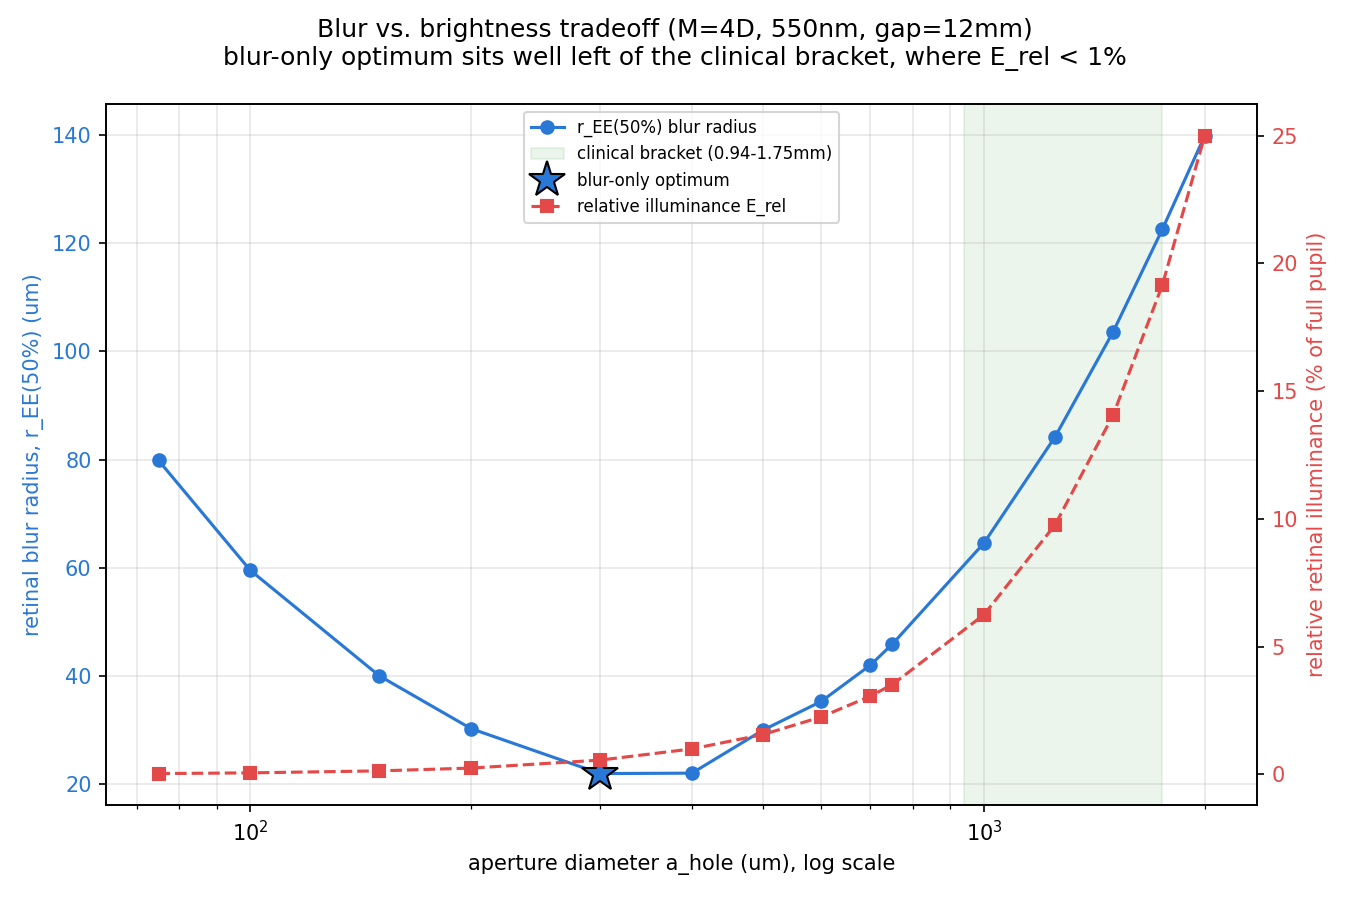
\includegraphics[width=0.7\textwidth]{figs/stage3a_fig1_blur_vs_brightness.png}
\caption{Blur radius and relative retinal illuminance vs.\ aperture, $M{=}4$D.
\texttt{stage3a\_fig1\_blur\_vs\_brightness.png}.}
\end{figure}
\begin{figure}[h!]
\centering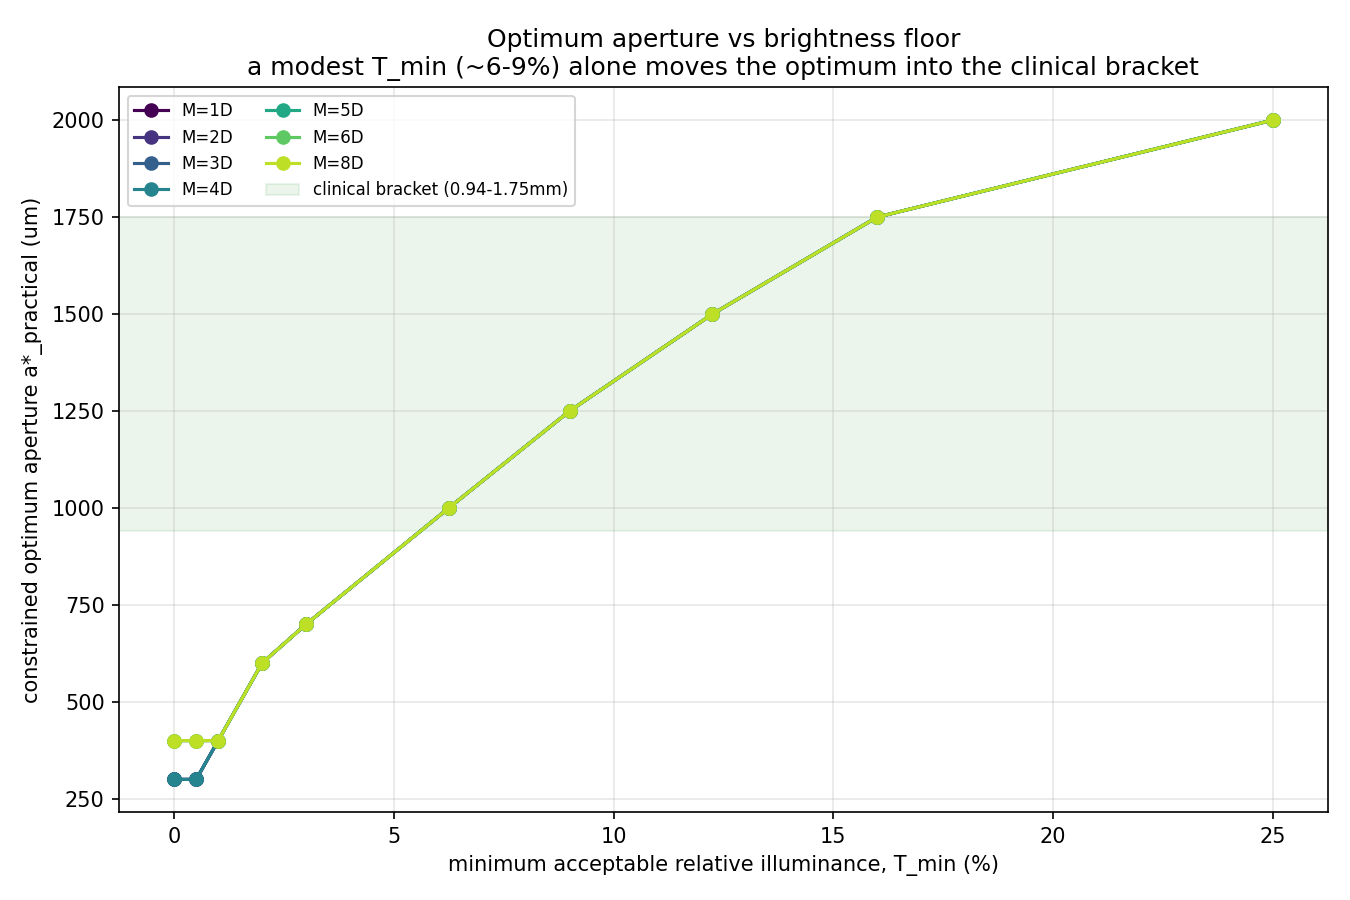
\includegraphics[width=0.7\textwidth]{figs/stage3a_fig2_optimum_vs_Tmin.png}
\caption{Constrained optimum aperture vs.\ $\Tmin$, all myopia levels; green band is the
clinical bracket. \texttt{stage3a\_fig2\_optimum\_vs\_Tmin.png}.}
\end{figure}
\begin{figure}[h!]
\centering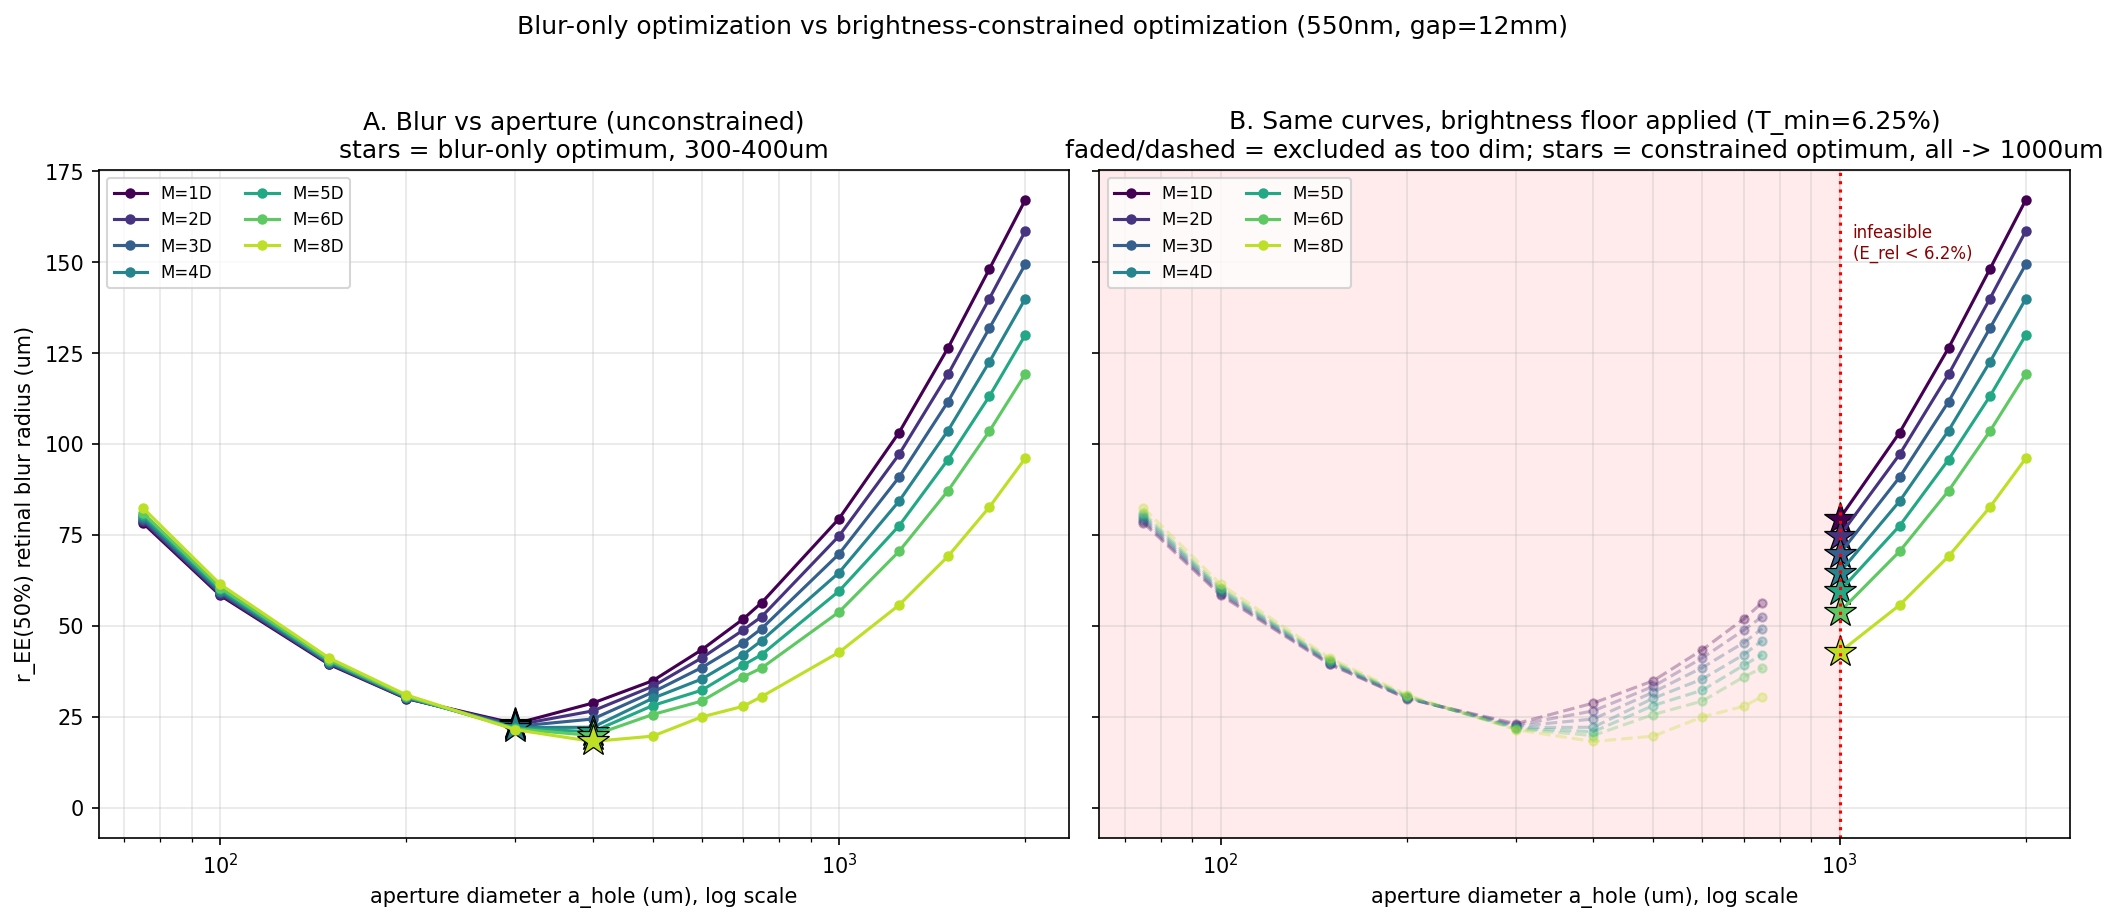
\includegraphics[width=0.7\textwidth]{figs/stage3a_fig4_blur_then_constraint.png}
\caption{Panel A: unconstrained blur-vs-aperture. Panel B: the same curves with the
$6.25\%$ floor applied. \texttt{stage3a\_fig4\_blur\_then\_constraint.png}.}
\end{figure}

\section{Percentile-choice robustness}
\label{sec:convergence}
$r_{EE}(70\%)$, extracted directly from the raw retinal field with no pipeline modification,
was combined with the pre-existing $50/80/90\%$ columns. Unconstrained, the four percentiles
disagree modestly ($300$--$400\,\mu$m for $50/70\%$; $400$--$600\,\mu$m for $80/90\%$). Once
the $6.25\%$ brightness floor is applied, \textbf{all four percentiles converge to exactly
the same answer -- $1000\,\mu$m -- at every myopia level}: the brightness floor matters far
more than which encircled-energy percentile is chosen.
\begin{figure}[h!]
\centering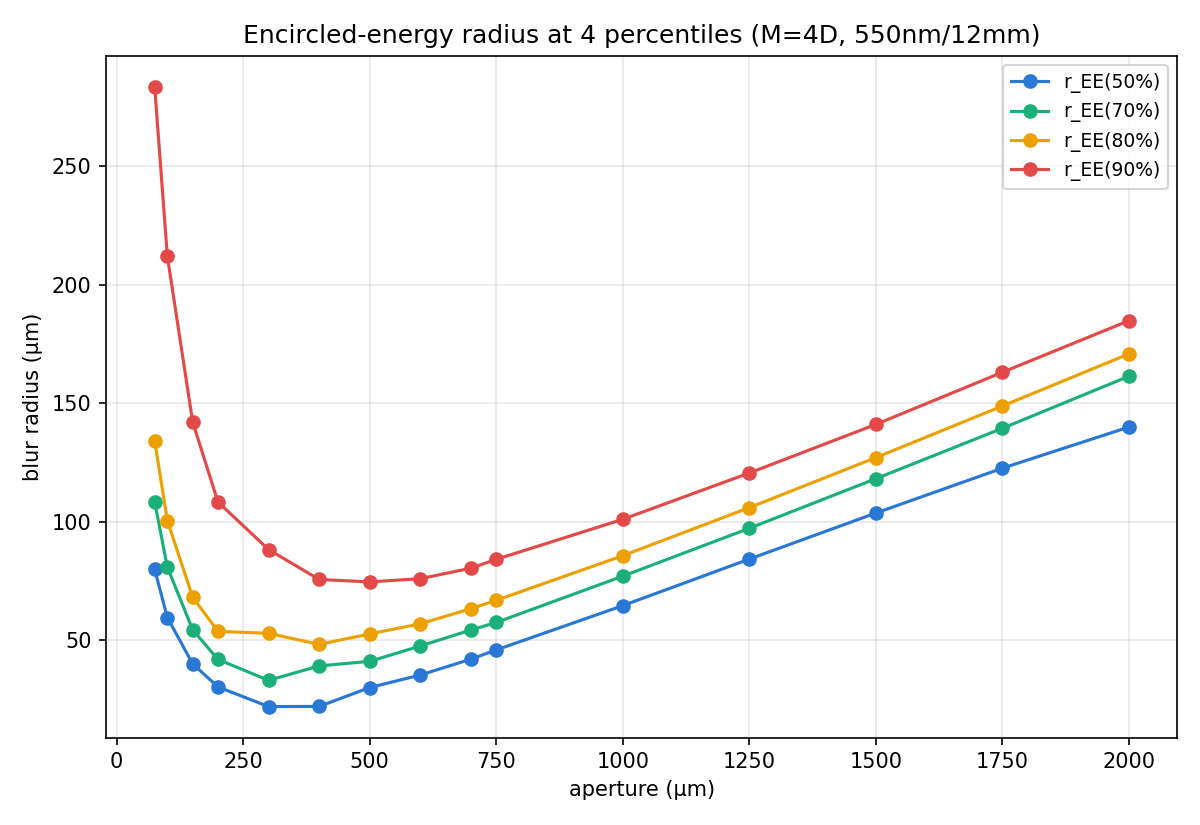
\includegraphics[width=0.7\textwidth]{figs/ee_all_percentiles.png}
\caption{$r_{EE}$ at $50/70/80/90\%$ vs.\ aperture, $M{=}4$D. \texttt{ee\_all\_percentiles.png}.}
\end{figure}

\section{Citation discipline}
\label{sec:litdiscipline}
Every implemented relationship in Handbook 2's comprehensive metric suite is classified as
\emph{first\_principles} (needs no citation -- energy conservation, the Fourier-optics
definition of MTF), \emph{published} (a specific named model, with any simplification
stated), or \emph{heuristic} (a simplified stand-in, e.g.\ where the full multi-parameter
Barten CSF could not be reproduced exactly). Twenty citation entries cover: the Strehl
ratio, MTF/OTF, the Airy diameter, F-number, RMS spot radius, the troland unit and CIE
photopic luminous efficacy, two CSF parametrizations, the Rose--DeVries law, Weber contrast,
the Blackwell (1946) foveal-detection dataset, MAR/Snellen conversion, the Visual Strehl
metric, the Stiles--Crawford effect, and ocular aberration magnitudes. This handbook's own
new material (Ch.~\ref{ch:array}--\ref{ch:vignetting}) follows the same discipline: the
Barten (1999) CSF (\S\ref{sec:riskmodel}) and the saccade-amplitude/center-bias literature
(\S\ref{sec:vigapply}) are both \emph{published}, explicitly distinguished from the
\emph{heuristic} \texttt{uniform} gaze-distribution placeholder they sit alongside.

\section{Photometric chain, MTF/CSF, and three independent acuity models}
The full chain from scene luminance to retinal photon flux reuses the standard
image-irradiance camera equation, $E_{\text{retina}}=\pi N\tau L_{\text{scene}}/[4(\text{F\#})^2]$,
with heuristic ocular transmission $\tau{=}0.90$ (range $0.85$--$0.95$) exposed as an
overridable argument. MTF is computed exactly (no free parameters) as
$|\mathcal F\{\text{PSF}\}|$, radially averaged. Two published CSF parametrizations are
implemented and deliberately never merged -- a band-pass model peaking near $4$ cyc/deg, and
the Mannos--Sakrison parametrization peaking near $8$ cyc/deg -- and their genuine
peak-location disagreement is reported as a finding, not resolved by picking one
(\S\ref{sec:errorbudget} above).

Three independent acuity models are computed and compared, never averaged into one number:
(1) MAR from the MTF50/MTF10 cutoff via $\text{MAR(arcmin)}=30/C$; (2) an approximate Visual
Strehl (VSX-style) metric, CSF-weighting actual vs.\ diffraction-limited MTF; (3) a
Rose--DeVries photon-noise-limited bound, $\text{MAR}\propto\Phi^{-1/2}$, calibrated to a
\emph{relative} noise-floor change, not an absolute clinical prediction.

\begin{figure}[h!]
\centering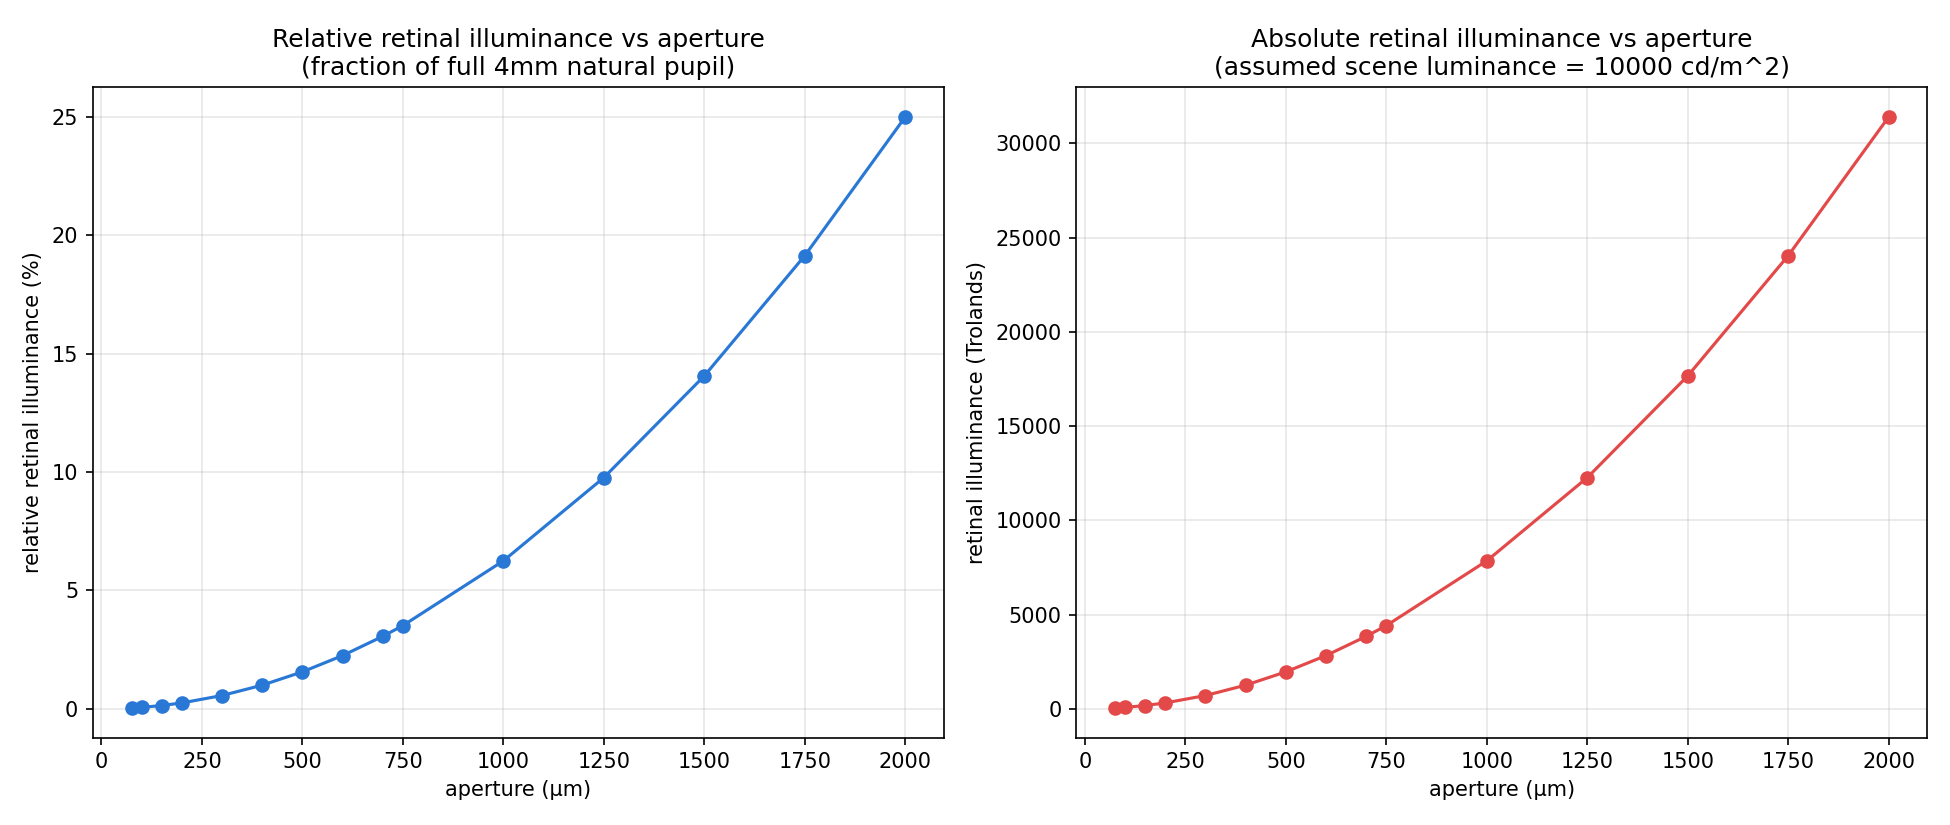
\includegraphics[width=0.85\textwidth]{figs/illuminance_troland.png}
\caption{Relative retinal illuminance and absolute Trolands vs.\ aperture, $M{=}4$D.
\texttt{illuminance\_troland.png}.}
\end{figure}
\begin{figure}[h!]
\centering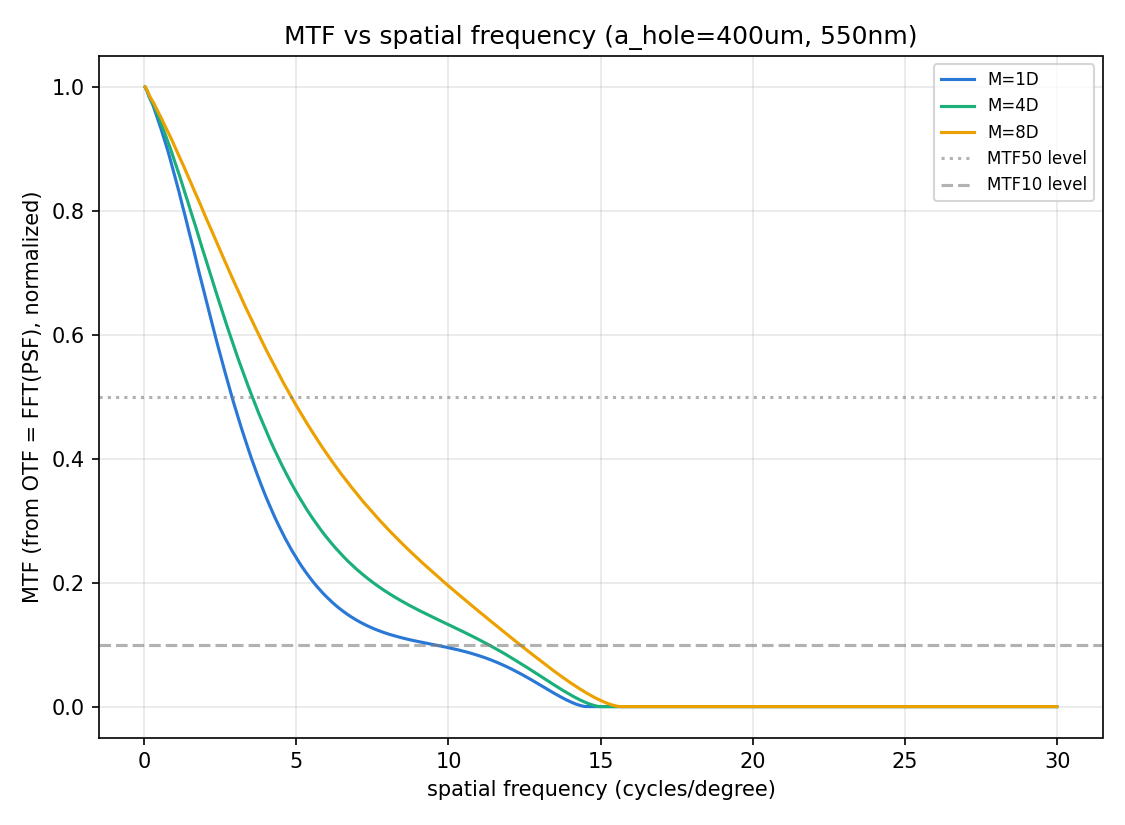
\includegraphics[width=0.85\textwidth]{figs/mtf_curves.png}
\caption{Radially-averaged MTF vs.\ spatial frequency, three myopia levels, MTF50/MTF10
marked. \texttt{mtf\_curves.png}.}
\end{figure}
\begin{figure}[h!]
\centering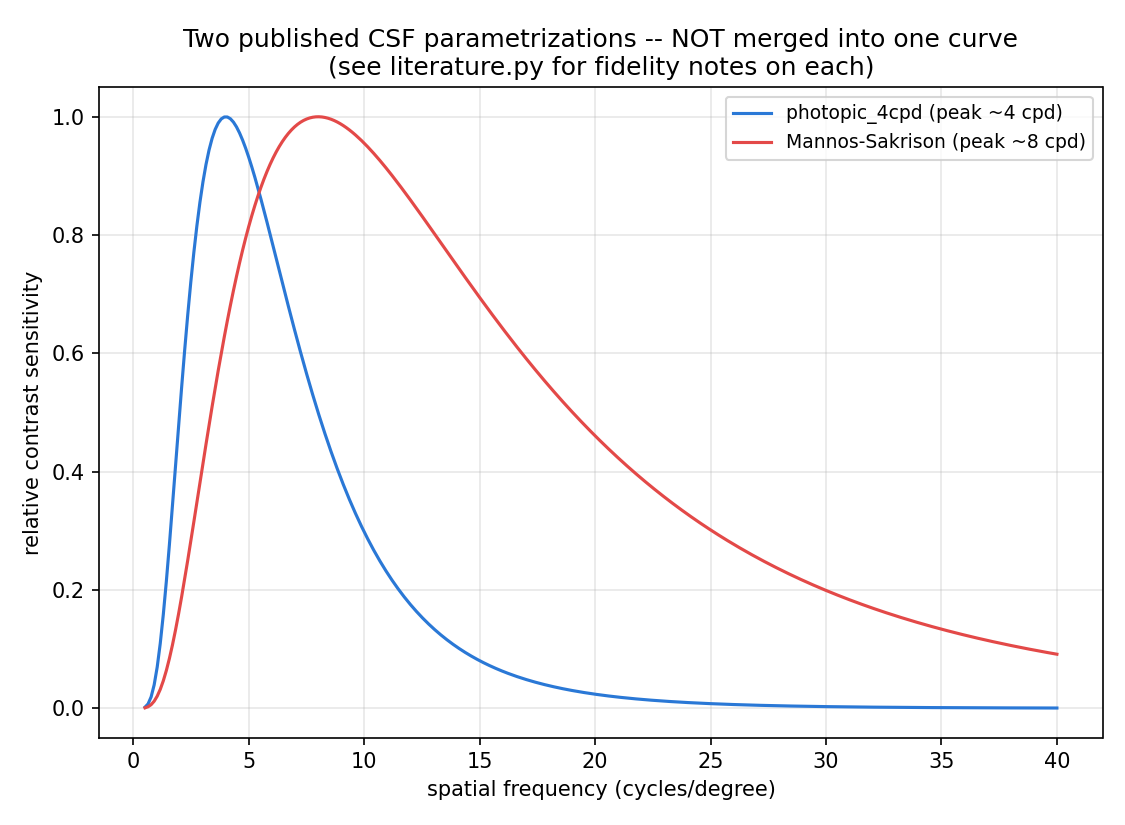
\includegraphics[width=0.7\textwidth]{figs/csf_comparison.png}
\caption{Two published CSF parametrizations, showing the genuine peak-location disagreement.
\texttt{csf\_comparison.png}.}
\end{figure}
\begin{figure}[h!]
\centering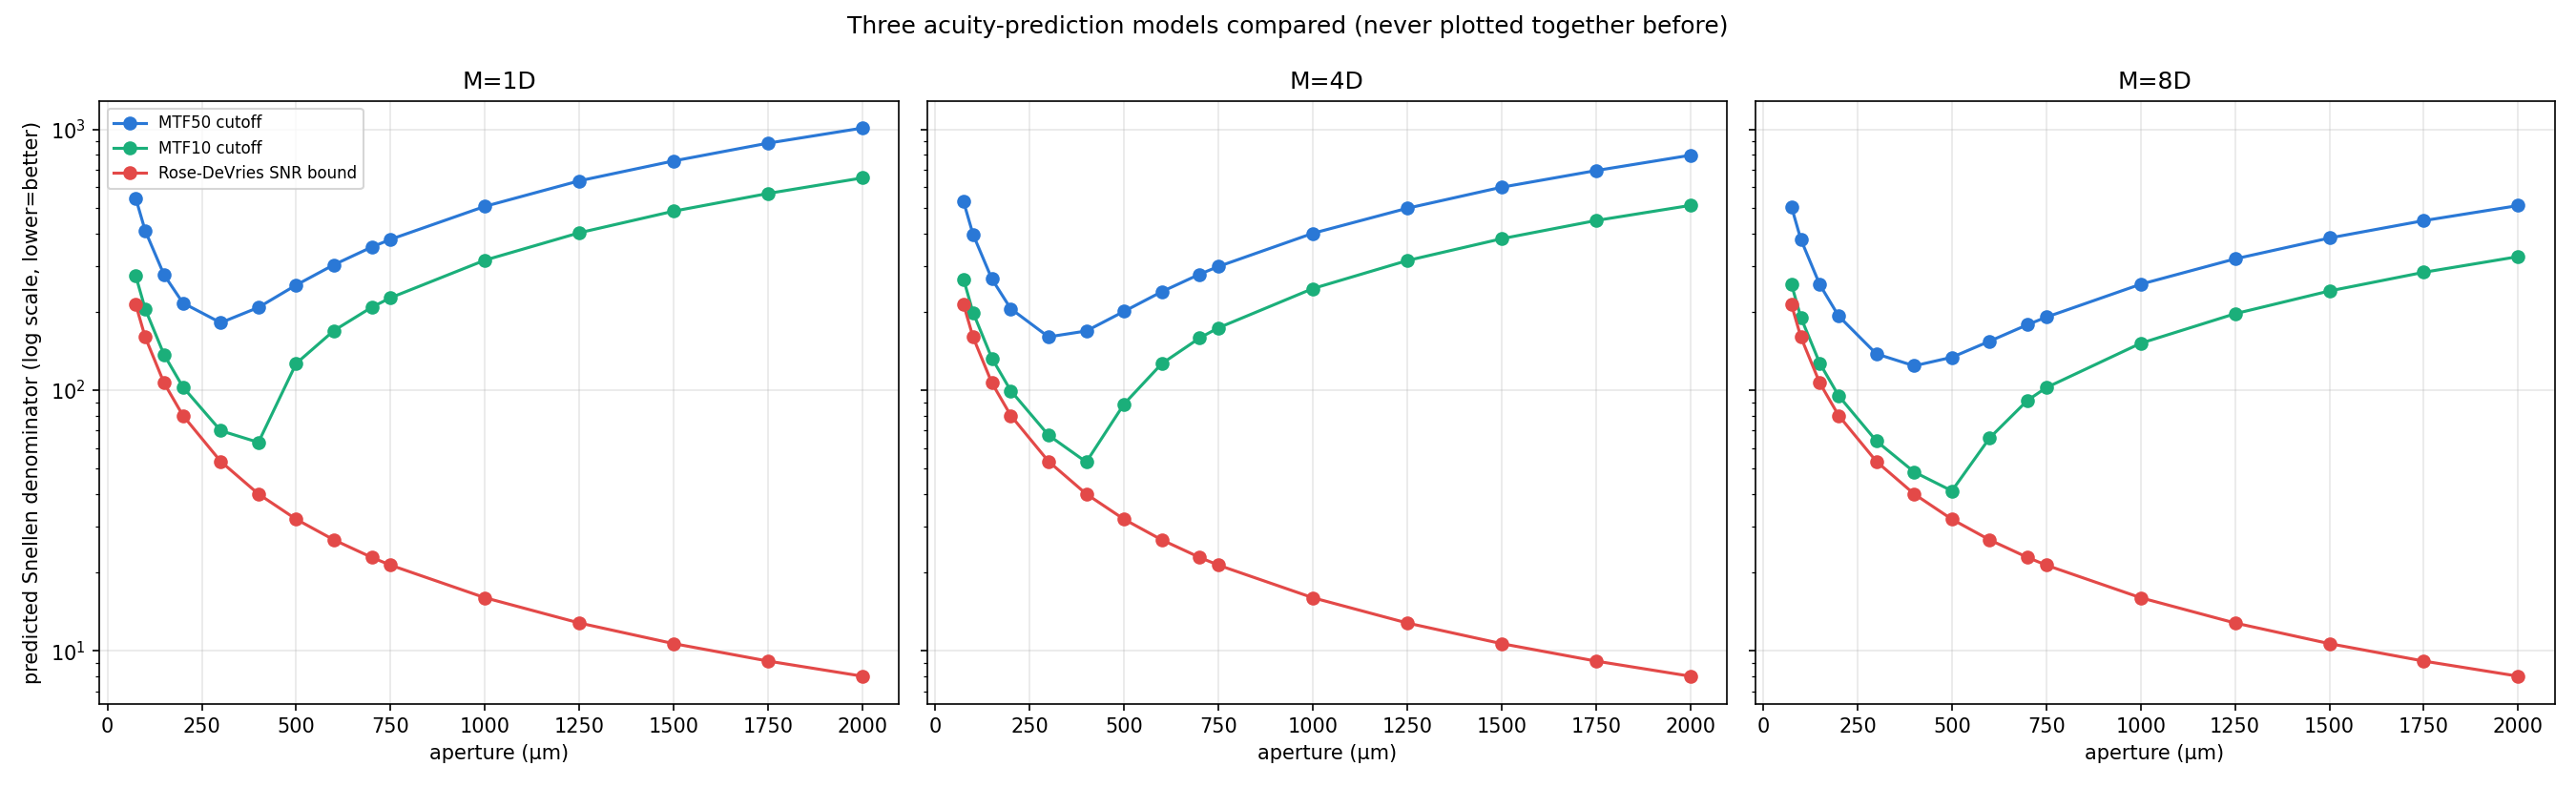
\includegraphics[width=0.85\textwidth]{figs/acuity_models_combined.png}
\caption{All three acuity-prediction models, per myopia level. \texttt{acuity\_models\_combined.png}.}
\end{figure}

\section{Sensitivity, validation, and Pareto fronts}
\begin{figure}[h!]
\centering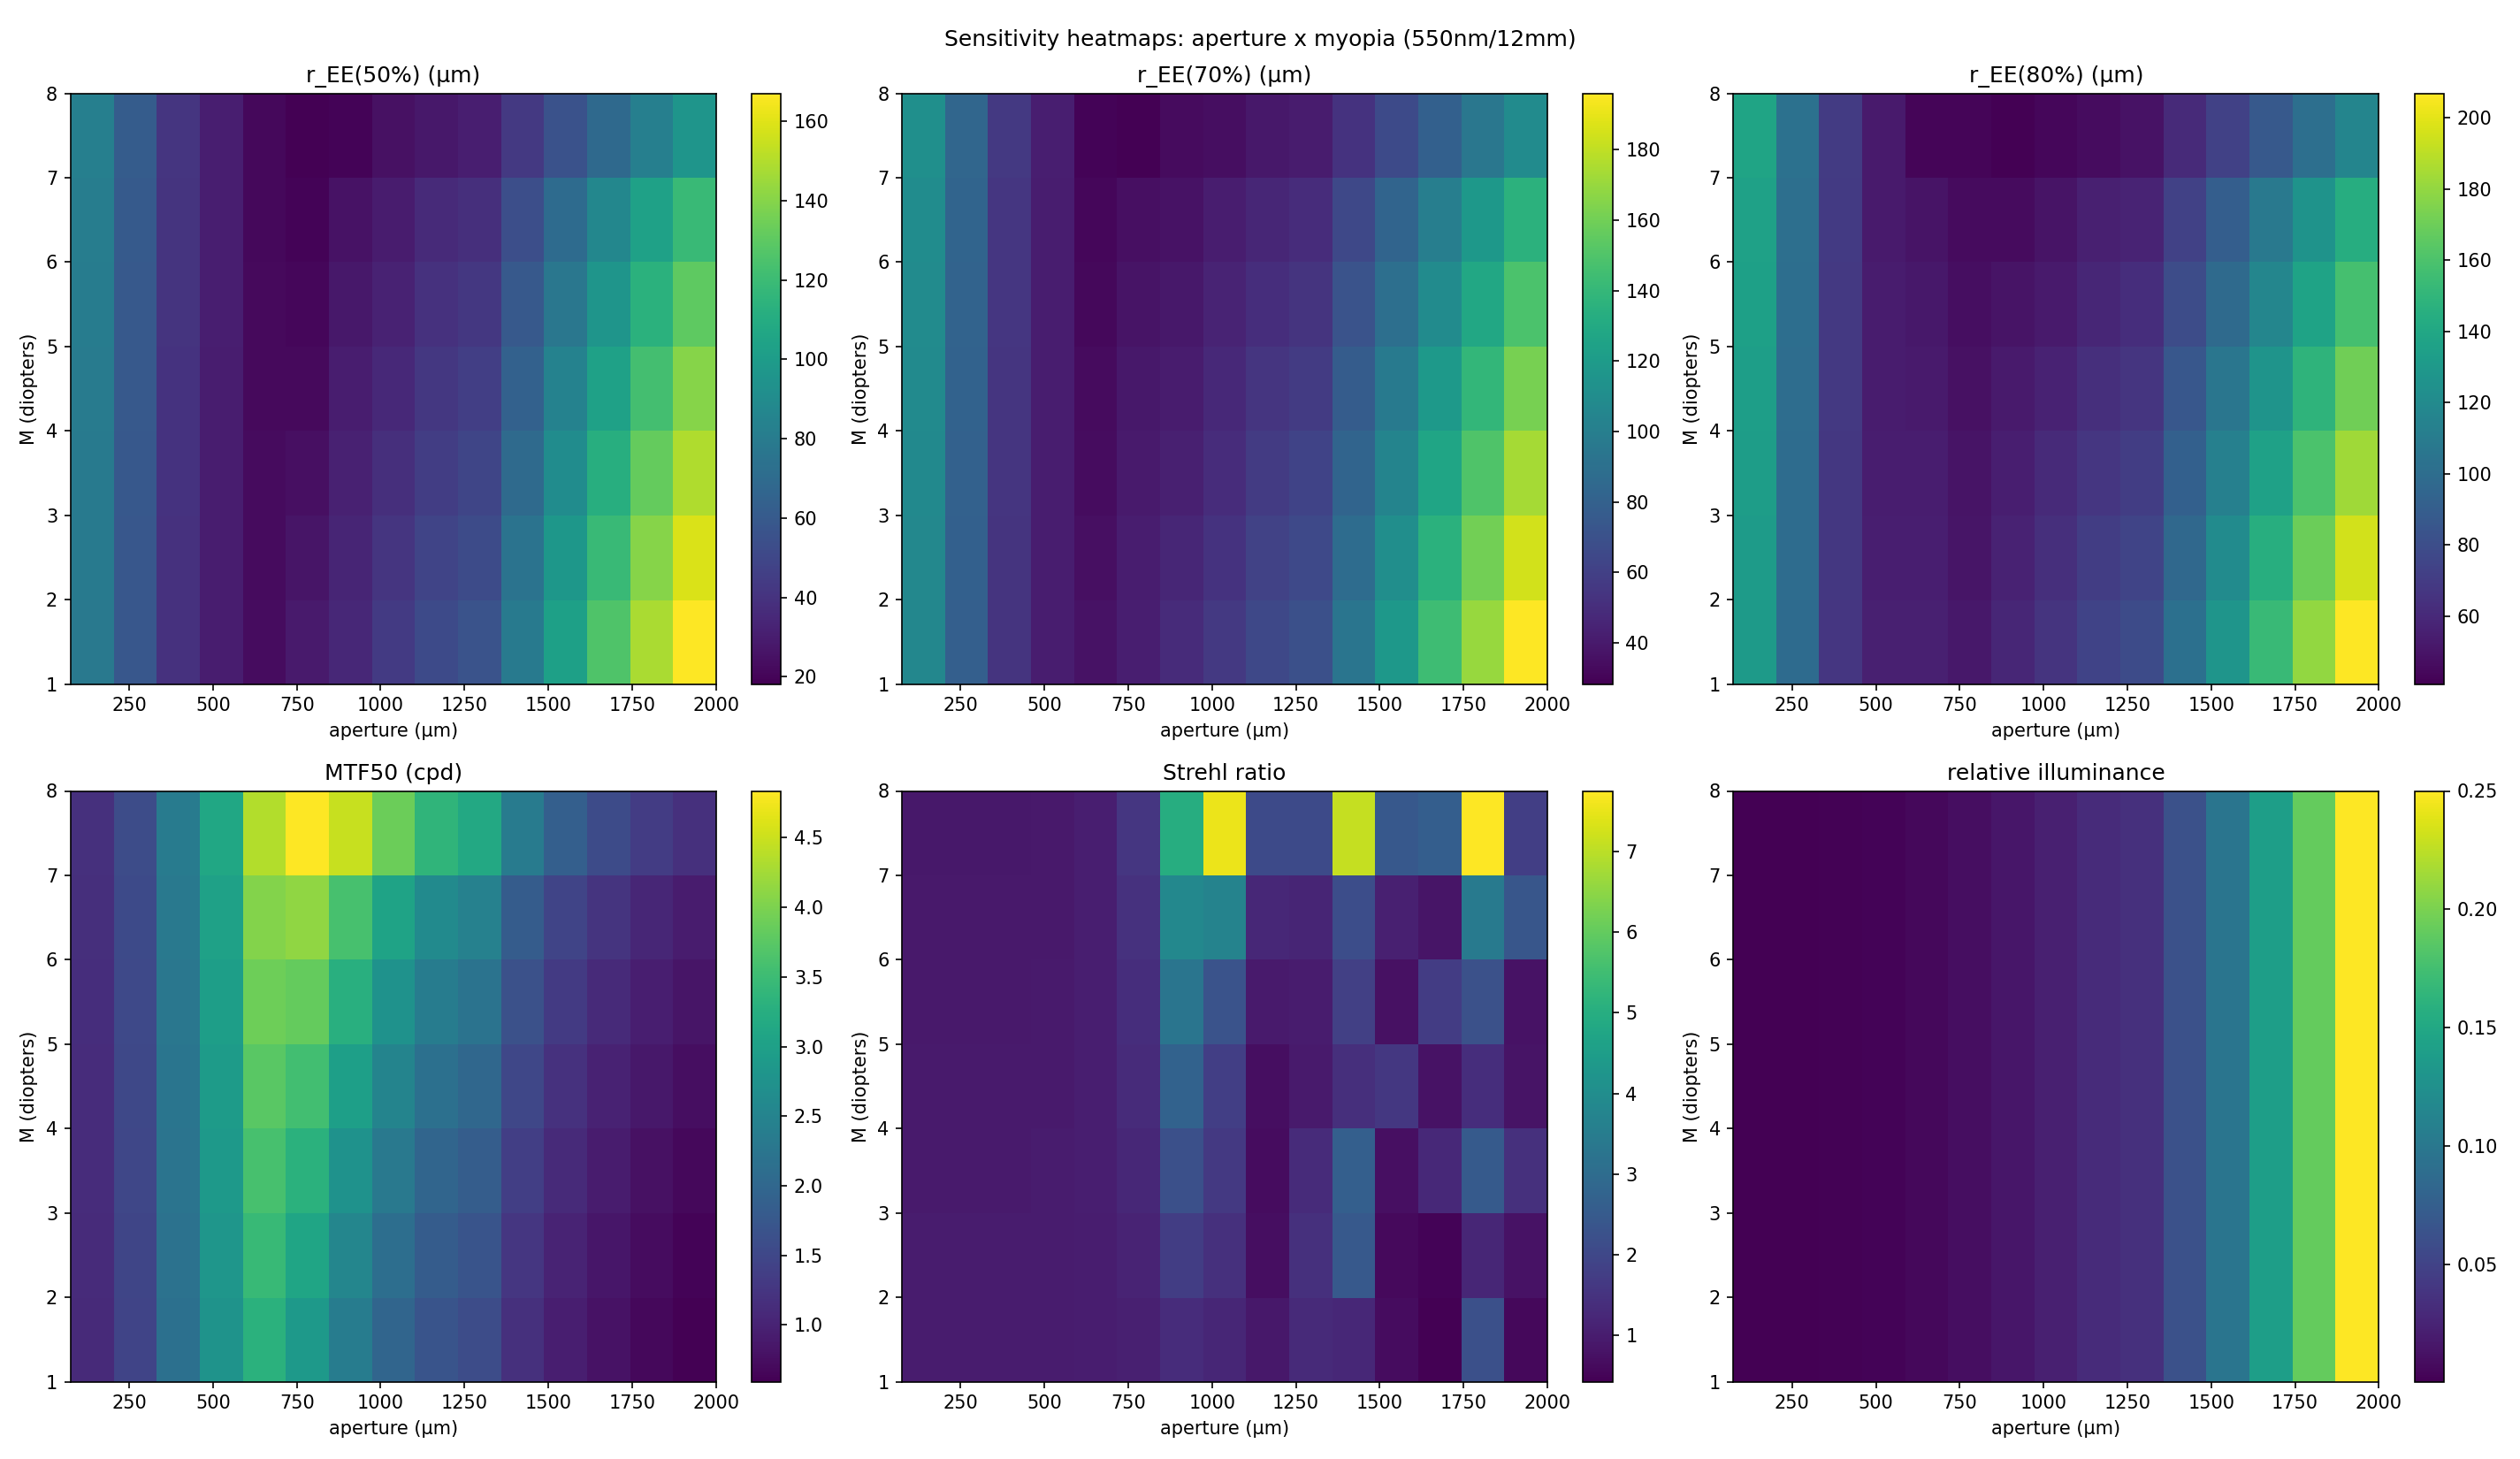
\includegraphics[width=0.85\textwidth]{figs/sensitivity_heatmaps_aperture_M.png}
\caption{Sensitivity heatmaps: aperture vs.\ myopia, for $r_{EE}(50\%)$, MTF50, Strehl, and
relative illuminance. \texttt{sensitivity\_heatmaps\_aperture\_M.png}.}
\end{figure}
\begin{figure}[h!]
\centering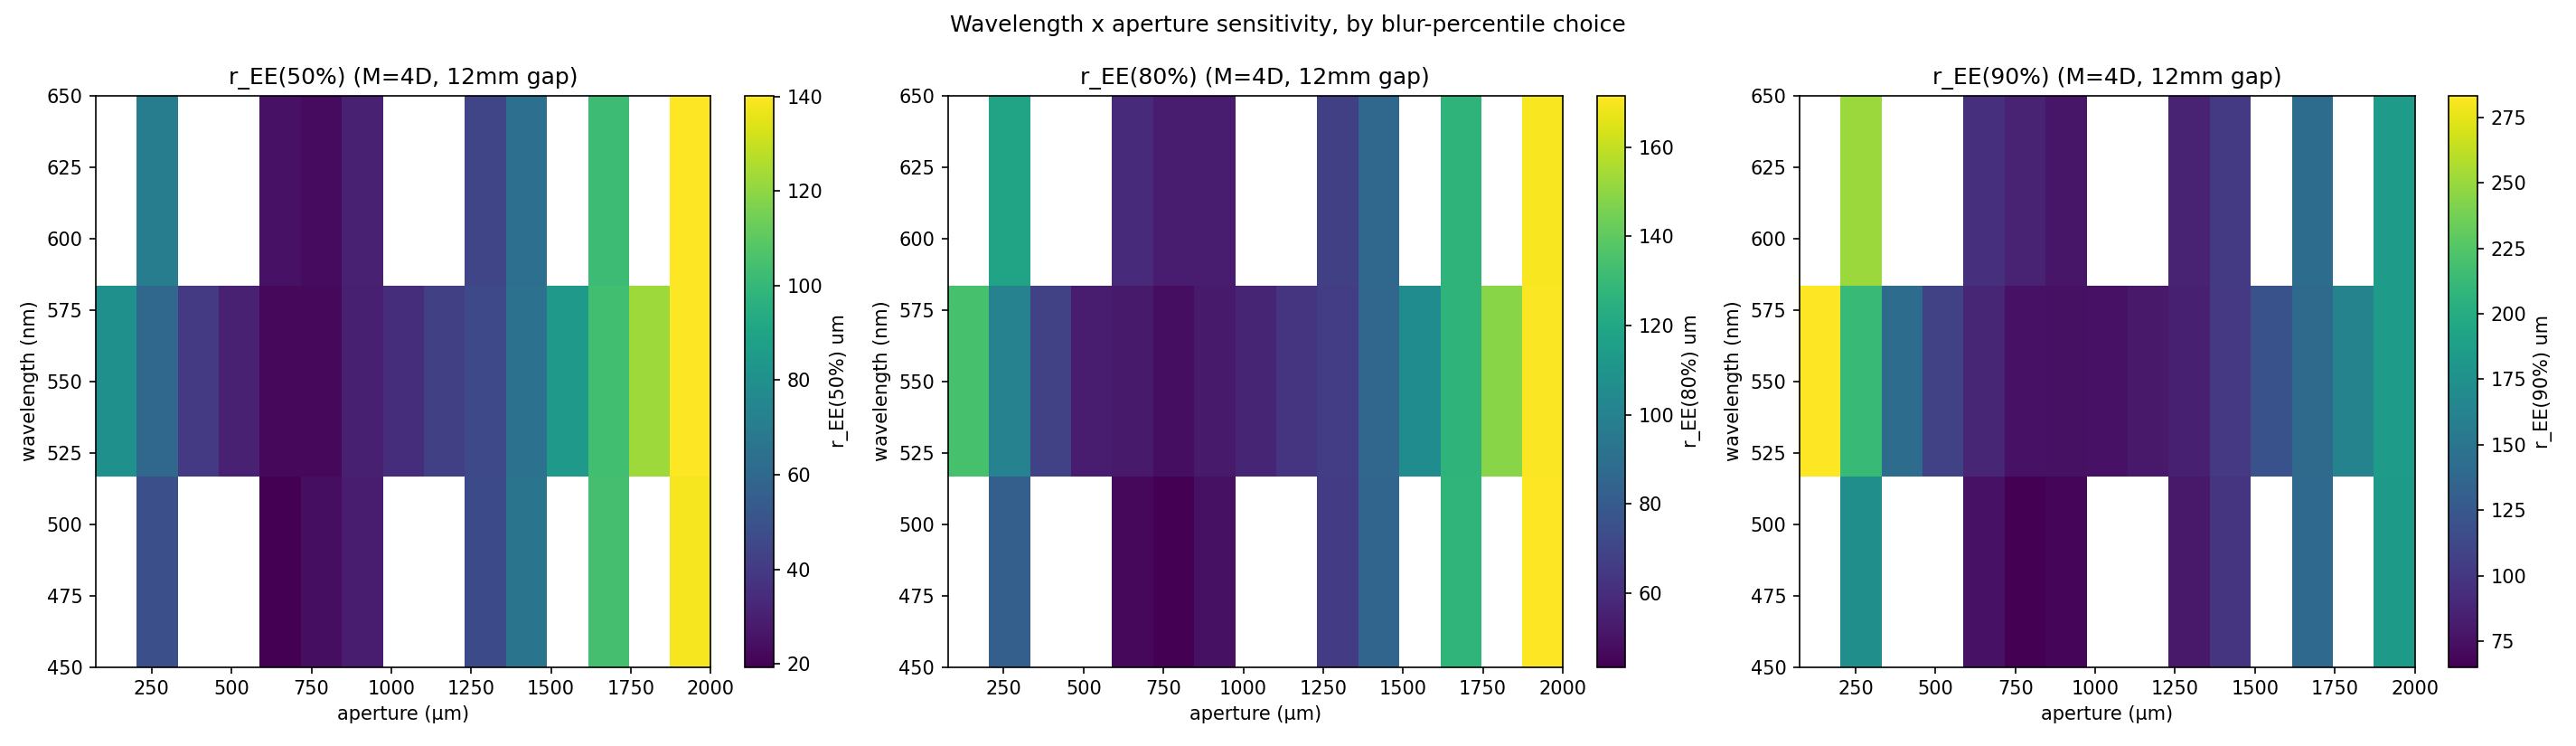
\includegraphics[width=0.75\textwidth]{figs/sensitivity_heatmap_wavelength_aperture.png}
\caption{$r_{EE}(50\%)$ sensitivity: wavelength vs.\ aperture, $M{=}4$D.
\texttt{sensitivity\_heatmap\_wavelength\_aperture.png}.}
\end{figure}
\begin{figure}[h!]
\centering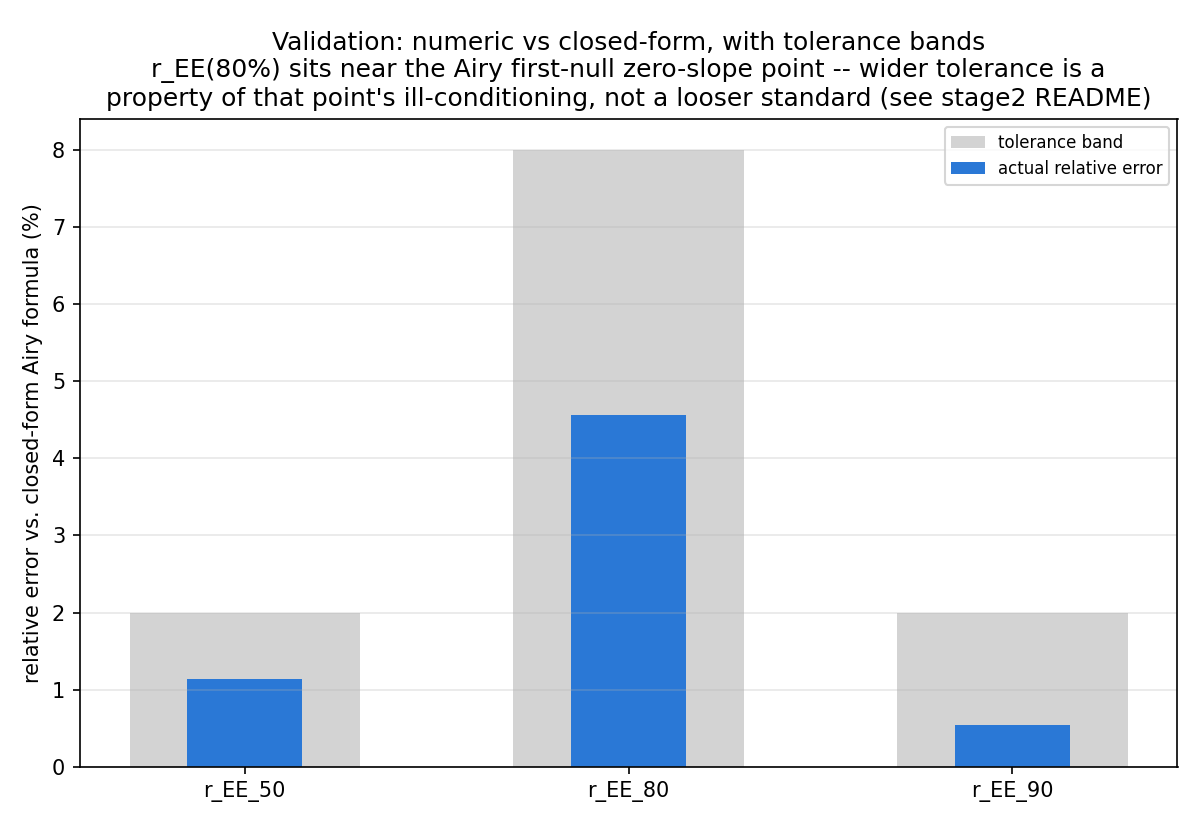
\includegraphics[width=0.7\textwidth]{figs/validation_tolerance_bands.png}
\caption{Numeric vs.\ closed-form Airy result, explicit tolerance bands per percentile.
\texttt{validation\_tolerance\_bands.png}.}
\end{figure}
\begin{figure}[h!]
\centering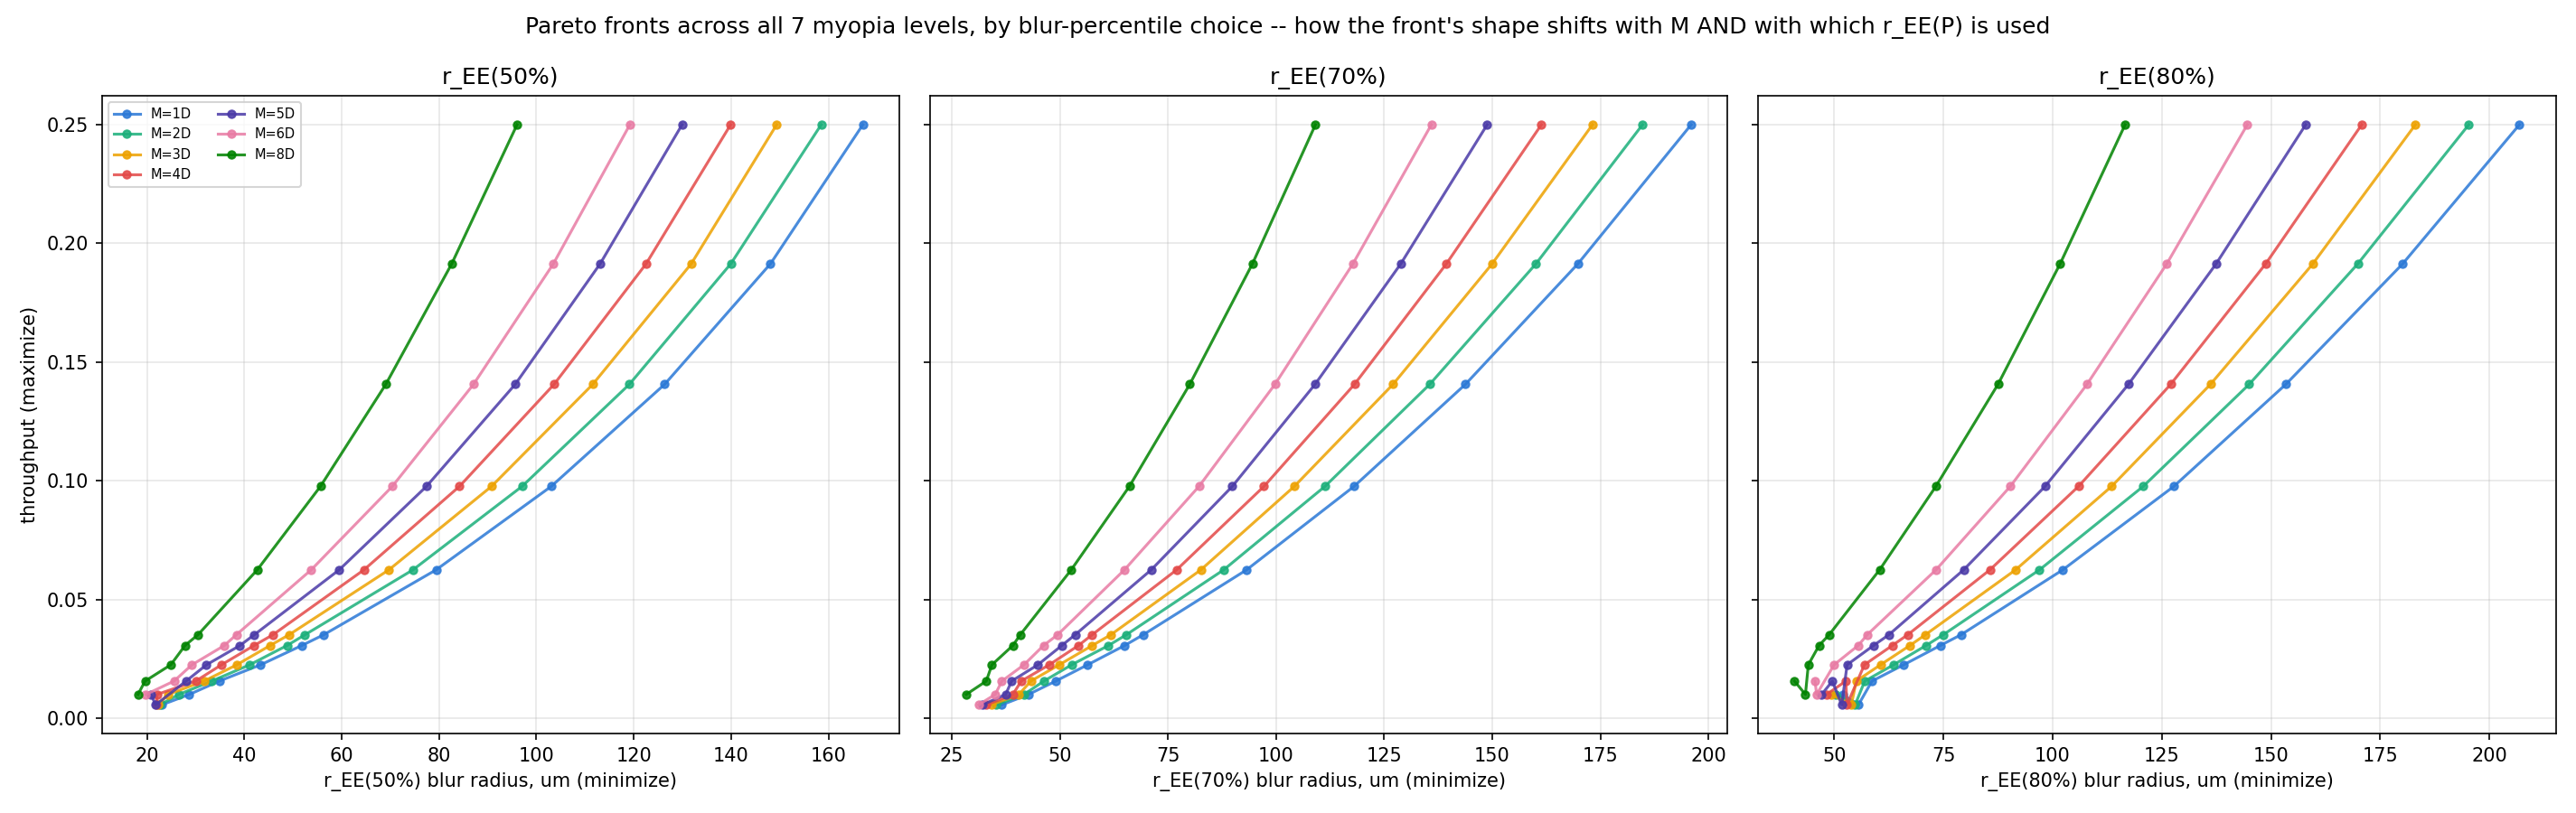
\includegraphics[width=0.7\textwidth]{figs/pareto_all_M_overlay.png}
\caption{Pareto-optimal fronts (blur radius vs.\ throughput), overlaid across all seven
tested myopia levels. \texttt{pareto\_all\_M\_overlay.png}.}
\end{figure}

\section{Model comparison: why the numbers disagree, diagnosed three ways}
\label{sec:modelcomparison}
Handbook 2's single most important synthesis result: an independent audit comparing three
implementations against each other and against real-world reference data, concluding that
disagreements across this project's own history, the deprecated closed-form formulas, real
clinical literature, and real patents have three distinct, individually-diagnosed causes --
not one broken model.
\begin{table}[h!]
\centering\small
\begin{tabular}{p{1.3cm}p{7.2cm}p{4.5cm}}
\toprule
\textbf{Model} & \textbf{What it computes} & \textbf{Basis} \\
\midrule
1 & Exact ASM, pinhole to cornea only. No eye, no myopia. & \texttt{stage1\_v2} \\
2 & Exact ASM$\times2$ + lens phase: full chain with axial myopia. & \texttt{stage2} \\
3 & The deprecated closed-form chain: $\aeff$, $\rgeo/\rdiff/\rtotal$ (RSS), $a^*$. & \texttt{classical\_formulas.py} \\
\bottomrule
\end{tabular}
\end{table}

\textbf{Finding 1 -- the old formula's accuracy depends entirely on which stage it is applied
at.} $\aeff$ was designed as a cornea-plane spot-size estimate, and there it tracks the exact
result reasonably well (Fig.~\ref{fig:comp-cornea}) -- consistently $14$--$24\%$ high, same
overall shape (see \S\ref{sec:r1result}'s table for the exact $13.8\%$/$23.7\%$ figures). The
much larger failure occurs when the same formula family is repurposed for retina-blur
optimization via RSS (\S\ref{sec:r1result}'s $64.8\%$/$192.8\%$) -- exactly the step
\S\ref{sec:asmfix} identifies as physically wrong. Root cause, confirmed by direct
calculation: $\aeff$ is itself non-monotonic at small apertures, producing a spurious
secondary dip around $100$--$150\,\mu$m unrelated to the true optimum
(Fig.~\ref{fig:comp-m4}).

\begin{figure}[h!]
\centering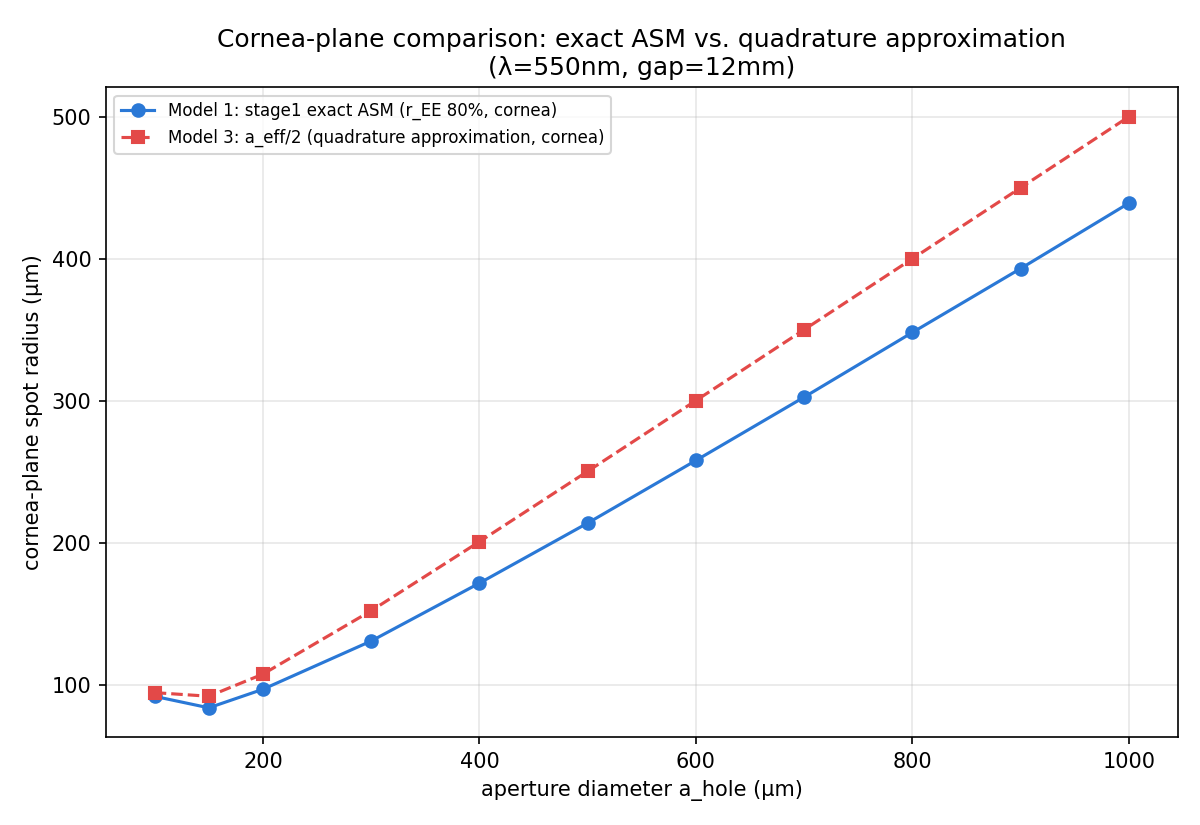
\includegraphics[width=0.7\textwidth]{figs/comparison_cornea.png}
\caption{Cornea-plane: old $\aeff/2$ vs.\ exact $r_{EE}(80\%)$. Biased high but correct
in shape.}
\label{fig:comp-cornea}
\end{figure}
\begin{figure}[h!]
\centering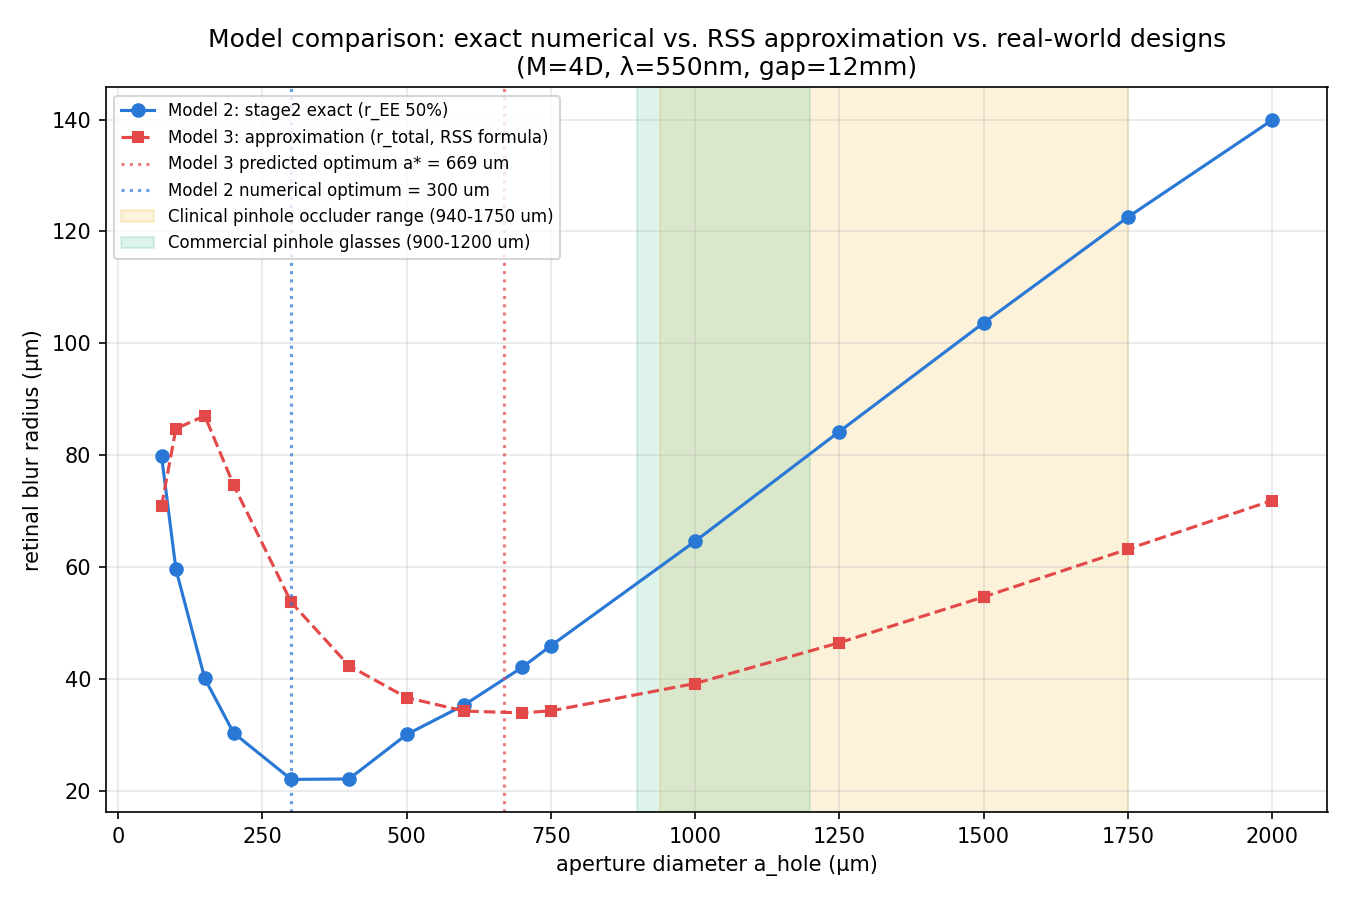
\includegraphics[width=0.7\textwidth]{figs/comparison_retina_M4.png}
\caption{Retina-plane, $M{=}4$D: old RSS $\rtotal$ vs.\ exact $r_{EE}(50\%)$, showing the
RSS formula's own spurious secondary dip near $100$--$150\,\mu$m.}
\label{fig:comp-m4}
\end{figure}

\textbf{Finding 2 -- none of the three physics models land near commercial/clinical
designs.}
\begin{table}[h!]
\centering\small
\begin{tabular}{lc}
\toprule
\textbf{Source} & \textbf{Aperture diameter} \\
\midrule
Model 2 (this project, $r_{EE}$ 50\%) & $300$--$400\,\mu$m \\
Model 3 (closed-form $a^*$) & $473$--$1339\,\mu$m \\
Rayleigh pinhole-camera formula, $d=1.9\sqrt{f\lambda}$ & $210$--$225\,\mu$m \\
Clinical pinhole occluders (optometry) & $940$--$1750\,\mu$m ($\sim1200\,\mu$m typical) \\
Commercial pinhole glasses & $900$--$1200\,\mu$m \\
\bottomrule
\end{tabular}
\end{table}
\begin{figure}[h!]
\centering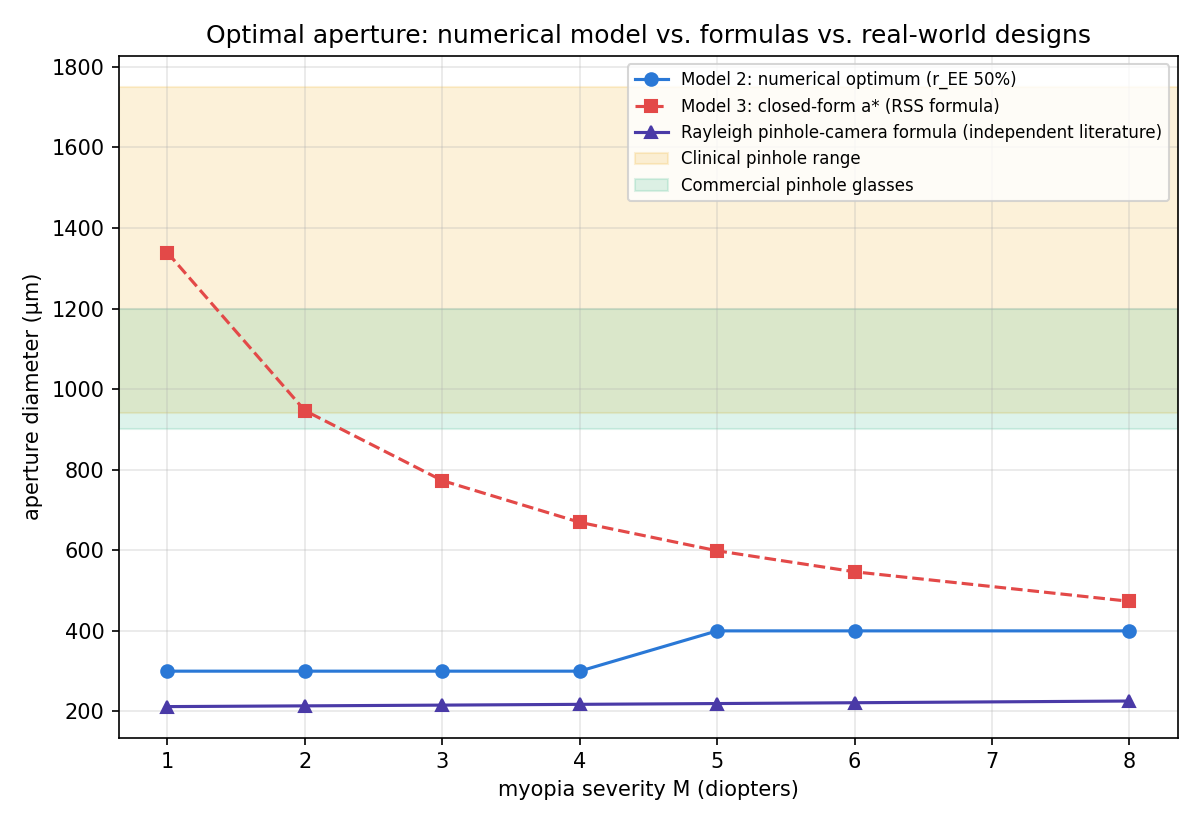
\includegraphics[width=0.7\textwidth]{figs/comparison_optimum_vs_rayleigh.png}
\caption{All five reference points on one axis. \texttt{comparison\_optimum\_vs\_rayleigh.png}.}
\end{figure}
All three physics-based results cluster in the $200$--$700\,\mu$m range, consistently
smaller than any commercial or clinical product. Diagnosed as scope, not error: every
physics model here optimizes blur \emph{alone}. A $300\,\mu$m hole passes roughly $16\times$
less light than a $1.2$mm hole (power $\propto d^2$), and none of the three compared models
builds in throughput. The brightness-constrained optimum
(\S\ref{sec:r1result}, $1000$--$1250\,\mu$m) is exactly the corrective step this finding
calls for.

\textbf{Finding 3 -- a genuine metric-selection error, confirmed against a real clinical
study.} Applying $\theta_{\text{blur}}=r_{EE}(P)/\vr$ literally at the same condition a real
clinical study measured ($1.2$mm aperture, $\sim5$D myopia, reported $\sim20/30$ Snellen,
$0.17$ logMAR):
\begin{table}[h!]
\centering\small
\begin{tabular}{lccc}
\toprule
\textbf{Metric} & \textbf{Value} & \textbf{Implied blur} & \textbf{Implied Snellen} \\
\midrule
$r_{EE}(50\%)$ & $73.8\,\mu$m & $10.45$ arcmin & $\sim20/209$ \\
FWHM (core-width) & $16.9\,\mu$m & $2.39$ arcmin & $\sim20/48$ \\
\bottomrule
\end{tabular}
\end{table}
$r_{EE}(50\%)$ predicts acuity nearly \textbf{seven times worse} than the clinical
measurement; FWHM lands within roughly $1.6\times$. Mechanism: $r_{EE}(50\%)$ is a
cumulative-\emph{energy} radius, counting diffuse peripheral light in faint outer Fresnel
rings that does not meaningfully impair letter recognition, while FWHM measures only the
bright, legibility-relevant core. This does not mean $r_{EE}(P)$ is wrong everywhere -- for
the blur-\emph{distribution} objective it is exactly the specified metric; it is specifically
wrong when repurposed, unmodified, for an acuity claim (\S\ref{sec:r7status},
\S\ref{sec:openr7}).

\section{Two confirmed anomalies, investigated rather than assumed away}
\textbf{Retina-plane FWHM ring-hopping}: FWHM jumps from $4.7\,\mu$m to $154.7\,\mu$m between
two adjacent $250\,\mu$m-spaced test apertures at $M{=}4$D -- over $30\times$. Retina-plane
FWHM is not a reliable single-value metric for this system.
\textbf{Strehl non-monotonicity}: a tenfold finer sweep, run specifically to test whether the
coarse sweep's non-monotonic Strehl-maximizing aperture was a discretization artifact,
revealed \emph{more} local maxima ($6$--$7$, not fewer) and \emph{larger} swings (up to
$8.4\times$, not smaller) -- the signature of genuine structure, not sampling noise.
\begin{figure}[h!]
\centering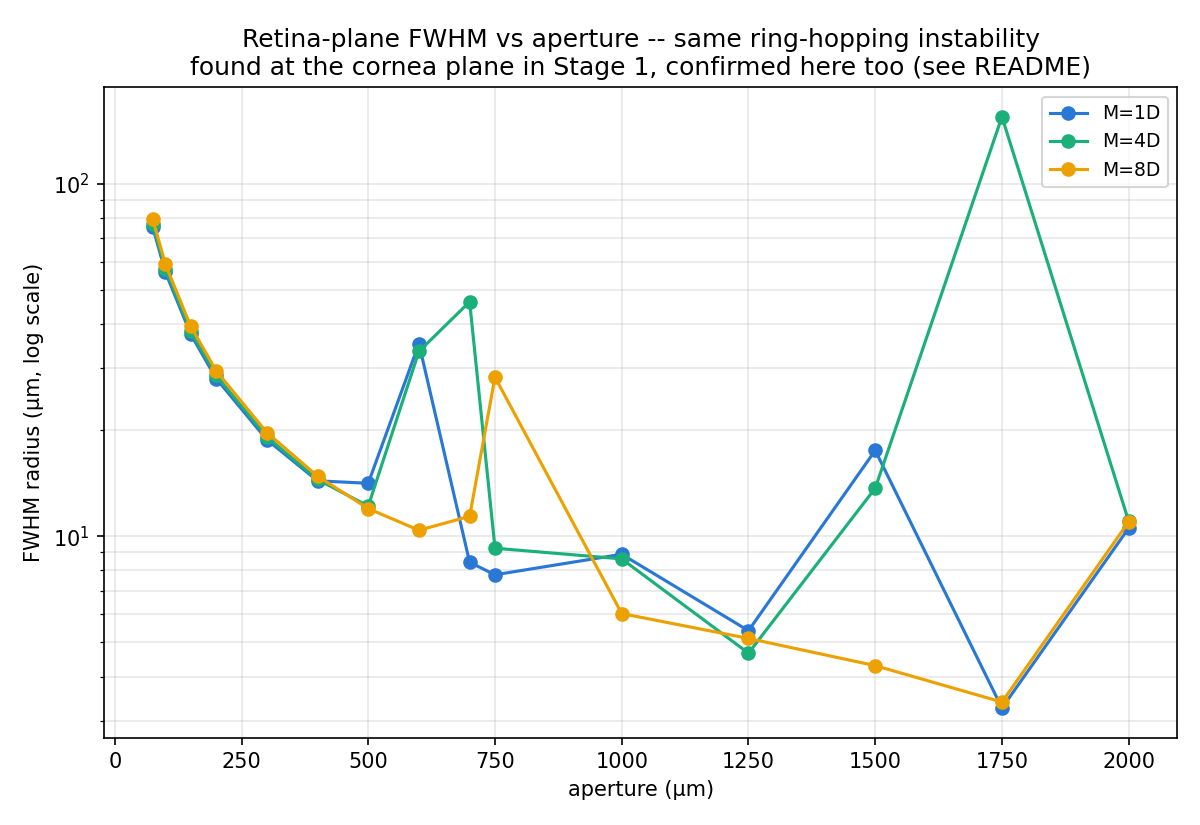
\includegraphics[width=0.7\textwidth]{figs/retina_fwhm_ring_hopping.png}
\caption{Retina-plane FWHM vs.\ aperture (log scale). \texttt{retina\_fwhm\_ring\_hopping.png}.}
\end{figure}
\begin{figure}[h!]
\centering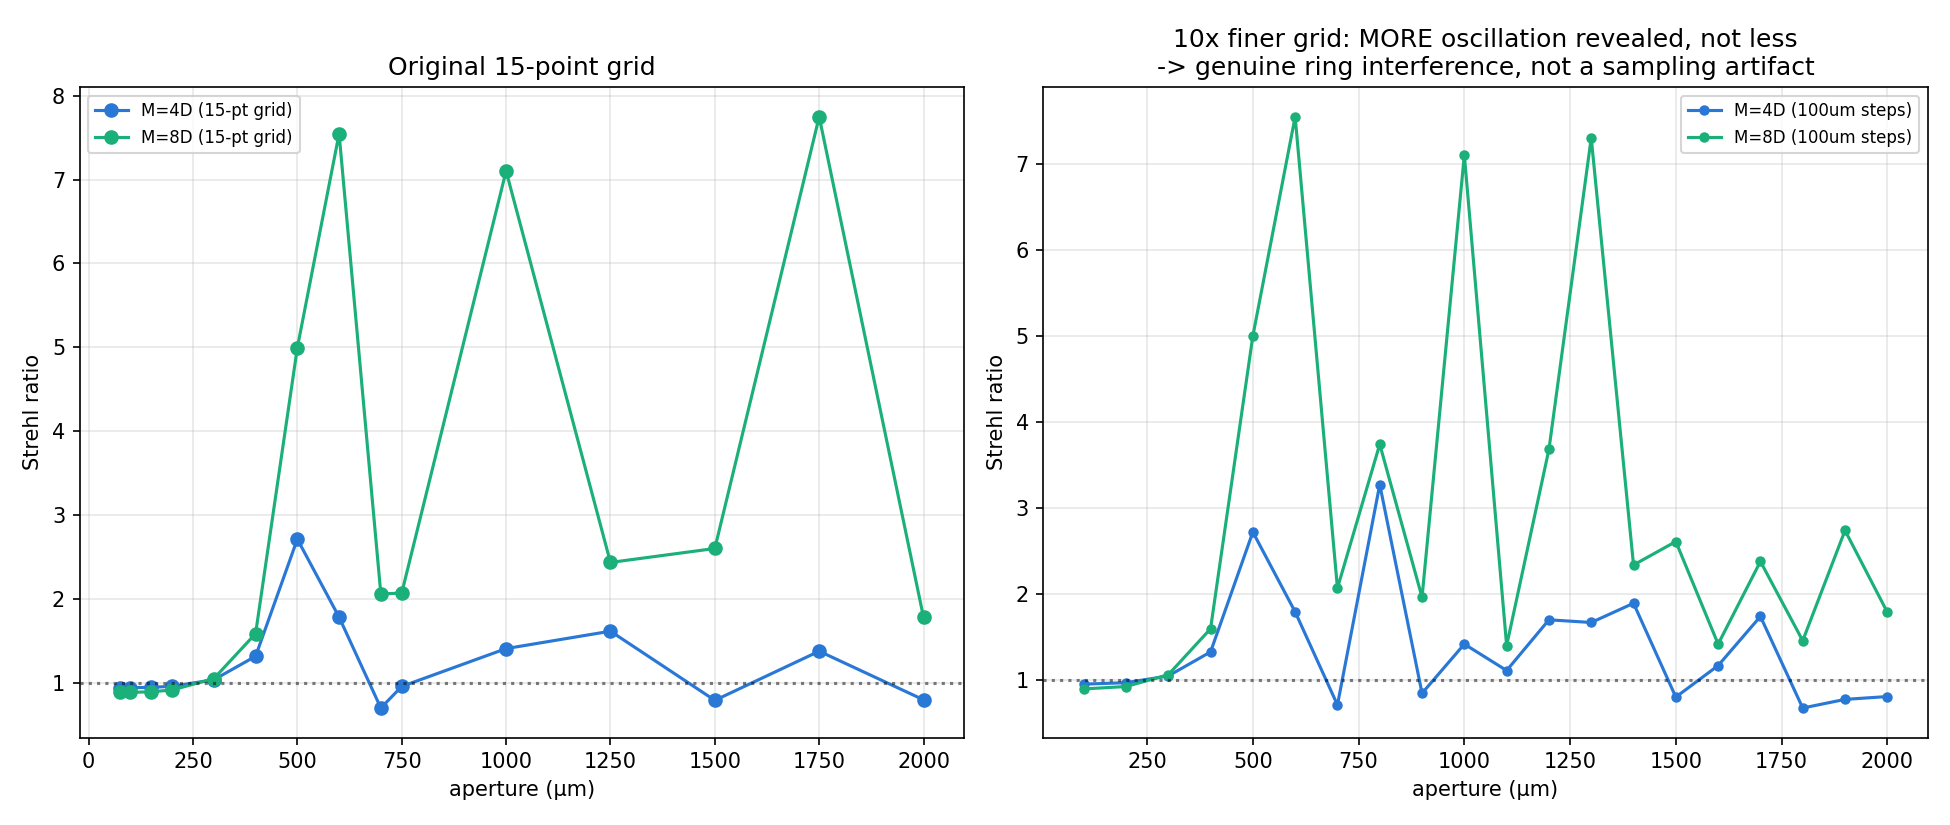
\includegraphics[width=0.85\textwidth]{figs/strehl_investigation.png}
\caption{Strehl ratio at coarse vs.\ tenfold-finer resolution -- the finer grid reveals
\emph{more} oscillation, not less. \texttt{strehl\_investigation.png}.}
\end{figure}

%======================================================================
\chapter{Array Design: Ghosting Theory}
\label{ch:array}
%======================================================================
Condensed from \texttt{Array\_Design/ghosting/THEORY.md}, \texttt{RESULTS.md}, and
\texttt{ANALYSIS.md}'s F1/F2 findings.

\section{Motivation: a contradiction between the original formula and real patents}
The original criterion (\texttt{stage\_array/array\_photometry.py}, moved unmodified to
\texttt{Array\_Design/photometry/array\_photometry.py}) called a design ``ghost-free'' if
$\Delta r$ (Eq.~\ref{eq:ghosting}, legacy) was smaller than the single-hole blur radius
$r_{EE}(P)$. Checked against two real, sold patents (KR 10-2081511, pitch $3.2$--$4.8$mm; CN
201716487U, pitch $0.7$--$1.2$mm; both $\dgap\!\sim\!12$mm, $\vr\!\sim\!22$--$24$mm), this
predicted severe violations ($30\times$--$400\times$) for \emph{both} -- the contradiction
that motivated re-deriving the formula at all.

\section{Literature grounding}
\begin{itemize}[nosep]
\item \textbf{Gabor superlens theory} (1941/2014): the closest existing precedent for a
quantitative multi-channel merging condition -- mismatched pitches in a two-array relay
cause channels to ``unite to form superfocal lines much smaller in number than the number of
microlenses.'' Cited as evidence this class of problem is solvable, not as a directly
transferable formula (it describes a two-array relay forming a real image, not a single
occluder imaged by the eye's own optics).
\item \textbf{Direct clinical evidence ghosting is real}: Kim, Park, Park \& Chun (2017, \emph{J
Korean Med Sci} 32(5):850--857) directly reports, in real subjects wearing real multi-pinhole
glasses, ``discomfort from after-images such as honeycomb images, horizontal grating, and
double or triple vision,'' significantly worse than single-pinhole glasses -- overturning the
original framing (real products \emph{do} report ghosting; the question is under what
conditions it becomes severe).
\item \textbf{An independent patent statement of the mechanism}: a separate US patent states,
independent of anything in this project, ``If two pinholes are separated by less than the
diameter of the pupil aperture, two pencils of ray$\ldots$form two retinal images. Further,
too large of a separation will result in dead spots$\ldots$while too small$\ldots$will
produce multiple images.'' A discrete precondition (are $\geq2$ holes simultaneously
illuminating the pupil) -- exactly the $\Neff$ quantity this project's own lattice
enumeration computes.
\item \textbf{Periodic-artifact visibility} (display-engineering ``screen-door effect''):
confirms the right framework -- express periodicity as cycles/degree, determine modulation
depth, compare against the human CSF threshold at that frequency.
\end{itemize}

\section{Reconciliation against real products}
\begin{table}[h!]
\centering\small
\begin{tabular}{p{2.6cm}p{2.0cm}p{1.6cm}p{2.4cm}p{4.5cm}}
\toprule
\textbf{Design} & \textbf{Pitch} & $\Neff$ & \textbf{Regime} & \textbf{Matches evidence?} \\
\midrule
KR 10-2081511 & $3.2$--$4.8$mm & $0$/$1.23$ & A & Consistent -- patent never discusses
ghosting \\
CN 201716487U & $0.7$--$1.2$mm & $23$--$28$ & B (untested) & Plausible, not independently
confirmed \\
Kim et al.\ 2017 MPH & pitch unstated & likely C & Danger zone & Directly matches real
reported symptoms \\
\bottomrule
\end{tabular}
\caption{This does not cleanly vindicate both patents -- it replaces one crude formula with
three separately-justified mechanisms and correctly locates where real problems are
reported.}
\end{table}

\section{The ghost-separation formula: found wrong, corrected, and independently validated twice}
\label{sec:deltar}
The formula originally in circulation,
\[
\Delta r = s\cdot \vr/\dgap \qquad \text{(legacy, Eq.~1)}
\]
does not vanish for an emmetropic eye: at $M{=}0$ it predicts ghost copies $1.86s$ apart in
an eye with zero defocus, which is not physically possible -- a perfectly focused eye images
a distant point to one point regardless of how many holes admit light. The corrected
expression,
\[
\Delta r = s\cdot\frac{|\vr-\vf|}{\vf} = \frac{s\cdot M}{P_0-M} \qquad \text{(corrected, Eq.~1$'$)},
\]
was derived three independent ways (paraxial ray transfer, wave-optics propagation, the
$M{=}0$ limit) in the original consolidation, and re-validated a second, independent time in
this handbook's own pipeline (Ch.~\ref{ch:optpipeline}, Stage 0): a genuine two-hole coherent
propagation plus an incoherent-sum reference, with $\Delta r$ measured by peak detection, not
formula lookup.

\begin{table}[h!]
\centering\small
\begin{tabular}{lcc}
\toprule
\textbf{Formula} & \textbf{Form} & \textbf{$R^2$ vs.\ 32 measured points} \\
\midrule
(a) legacy & $\Delta r = s\vr/\dgap$ & $-1701.71$ \\
(b) corrected & $\Delta r = sM/(P_0-M)$ & $0.9951$ \\
(c) free fit & $\Delta r = A[sM/(P_0-M)]+B$ & $0.9968$, $A{=}1.041$, $B{=}-2.75$ \\
\bottomrule
\end{tabular}
\caption{Ghost-formula validation, \texttt{array\_optimization/stage0\_ghost\_validation/ghost\_formula\_validation.csv}.
The free fit independently rediscovers (b) within its own pre-registered 5\% consistency band.}
\end{table}

\section{The continuous risk model, replacing binary Regime A/B/C}
\label{sec:riskmodel}
\texttt{ghosting\_regime.py}'s original Regime A/B/C classifier reads its worst case off the
\emph{minimum} $\Neff$ over pupil alignment -- correct for brightness (fewest holes =
darkest) but wrong for ghosting (most holes = worst ghosting). At $D_{\text{pupil}}{=}4$mm,
square packing, pitch $2500\,\mu$m is classified Regime A (``no second hole'') while carrying
$P(\Neff{\geq}2){=}0.82$ -- two or more holes active 82\% of the time. Only pitches above
$s_{\text{solo}}\approx3.94$mm (square) / $4.00$mm (hex) -- where even the \emph{maximum}
$\Neff$ is 1 -- are ghost-free by geometric construction.

\texttt{array\_optimization/stage2\_classification/classify.py} replaces the binary gate with
\[
\text{risk} = P(\Neff\geq2)\times\text{worst-harmonic perceptual margin},
\]
risk $=1.0$ being the point where the probability-weighted margin crosses the Barten (1999)
CSF detection threshold. The old binary label is still computed and exposed for reference,
never gated on.

\section{Harmonic series: what actually turned out to matter}
Ghosting theory's four-pass history (\texttt{ghosting/RESULTS.md}) found, then partly
un-found, a harmonic-series effect:
\begin{itemize}[nosep]
\item Pass 1 (heuristic CSF): zero Regime C found, an artifact of a CSF model evaluated far
outside its fitted range.
\item Pass 2 (real Barten 1999 CSF): reverses this completely -- 20/20 previously-``safe''
dense points reclassified Regime C.
\item Pass 3 (harmonic extension, legacy $\Delta r$): found the worst-case harmonic is
\emph{never} $n{=}1$ -- up to $n{=}20$, margin $4.4\times$ the fundamental-only estimate.
\item Pass 4 (harmonic extension, \emph{corrected} $\Delta r$): Pass 3's headline finding does
\textbf{not survive}. With the corrected formula the fundamental already sits at
$2.9$--$8.3$ cpd, at or past the CSF peak, so the worst harmonic is $n{=}1$ at
\textbf{20/20} dense points tested, worst-margin$\div$fundamental-margin $=1.000$ exactly.
\end{itemize}
This project's own record therefore directly contradicts a claim that ``the dangerous
harmonic is usually $n{=}2$--$3$'': under the validated formula it is $n{=}1$
essentially everywhere in this project's geometry, not a higher harmonic.

\begin{figure}[h!]
\centering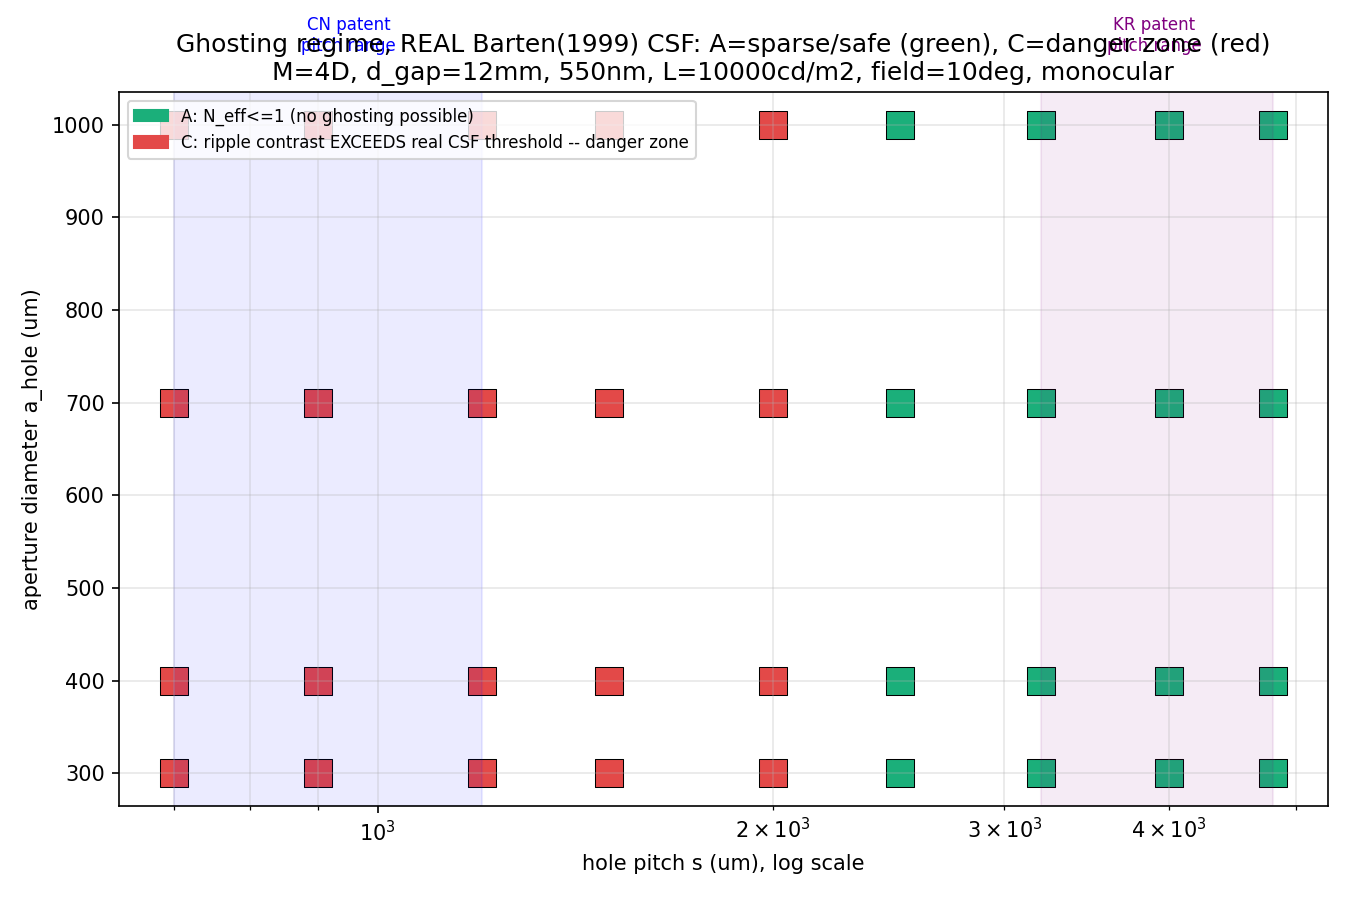
\includegraphics[width=0.85\textwidth]{Array_Design/ghosting/ghosting_regime_map_barten.png}
\caption{Regime map under the real Barten (1999) CSF (Pass 2). \texttt{ghosting/ghosting\_regime\_map\_barten.png}.}
\end{figure}
\begin{figure}[h!]
\centering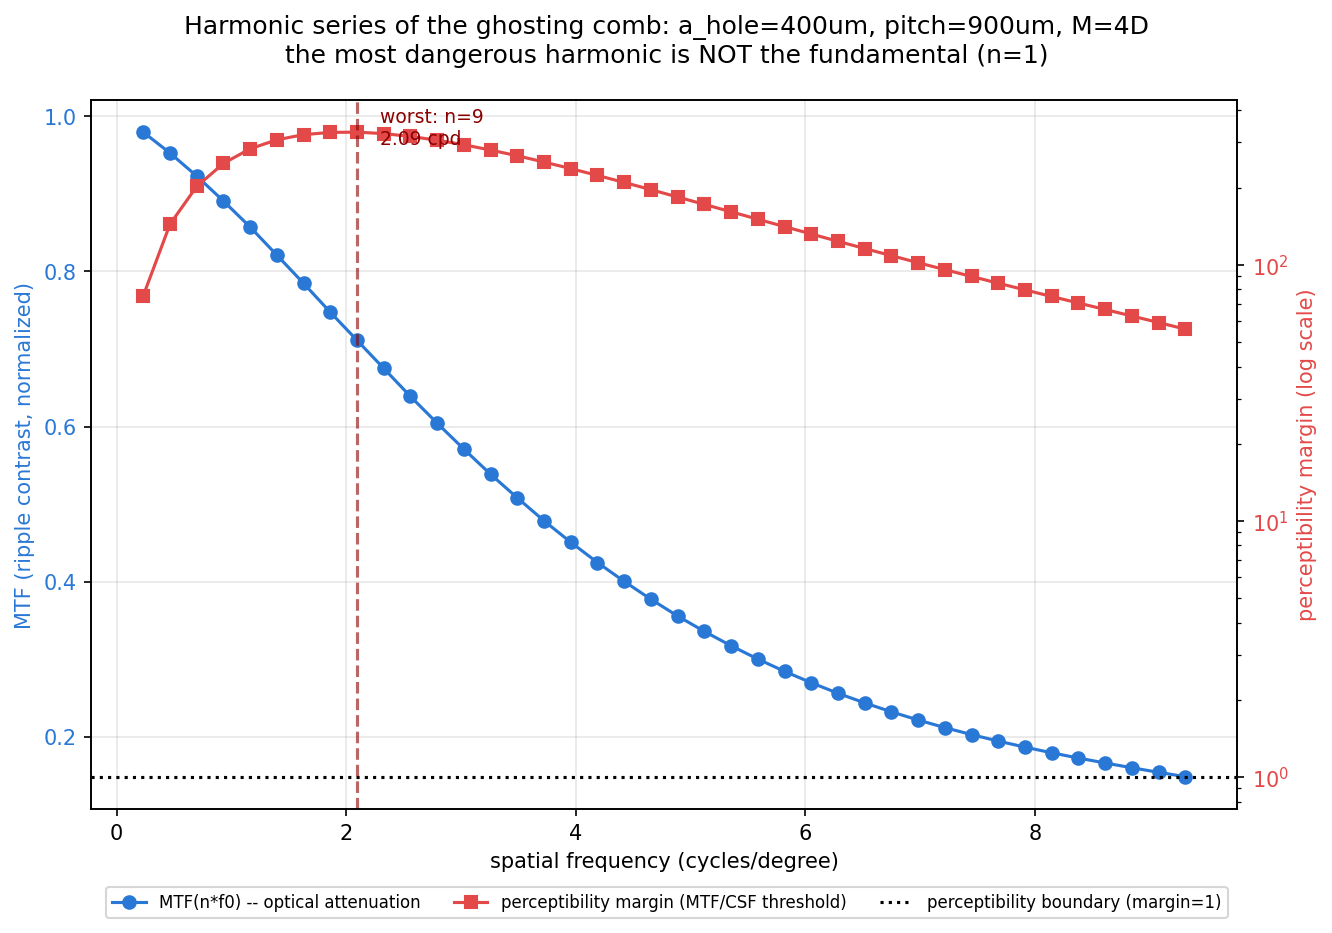
\includegraphics[width=0.85\textwidth]{Array_Design/ghosting/harmonic_margin_profile.png}
\caption{Harmonic margin profile (Pass 3, legacy formula -- superseded by Pass 4's
$n{=}1$ finding, kept for the historical record). \texttt{ghosting/harmonic\_margin\_profile.png}.}
\end{figure}
\begin{figure}[h!]
\centering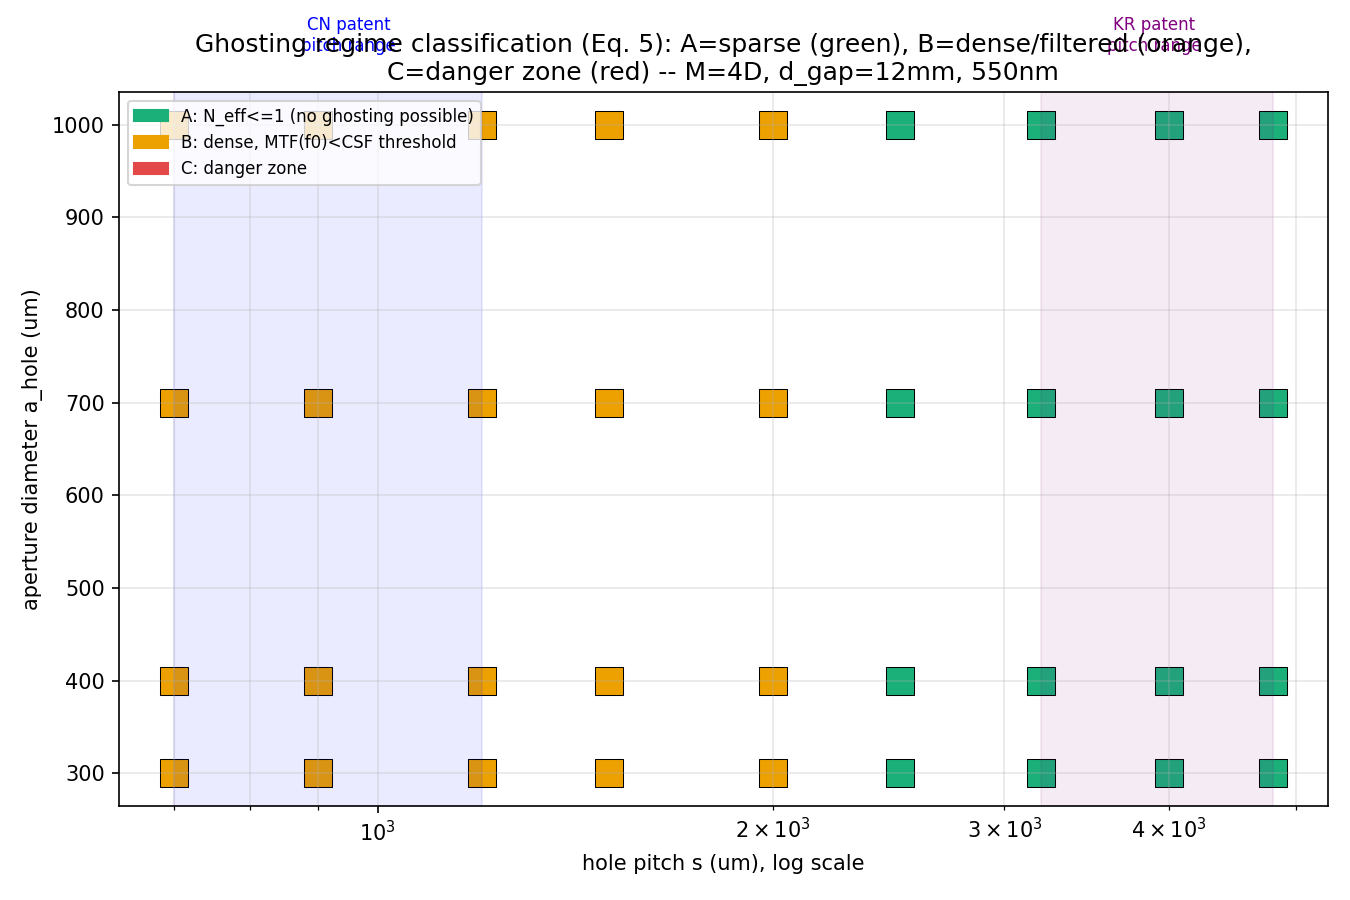
\includegraphics[width=0.85\textwidth]{Array_Design/ghosting/ghosting_regime_map.png}
\caption{Regime map, heuristic CSF (Pass 1) -- superseded by the Barten map above, kept for
the historical record of why Pass 1 found zero Regime C. \texttt{ghosting/ghosting\_regime\_map.png}.}
\end{figure}

\section{The N\texorpdfstring{$_{\text{eff}}$}{eff} alignment resolution problem (F3)}
A second, independent problem was found alongside F1/F2: \texttt{n\_holes\_exact\_sweep\_alignment()}
defaults to 25 offsets per axis; \texttt{ghosting\_regime.py} calls it with 15. Both are too
coarse exactly where the design boundary sits, and both err optimistic:
\begin{table}[h!]
\centering\small
\begin{tabular}{lccc}
\toprule
\textbf{pitch ($\mu$m)} & \textbf{quantity} & \textbf{$n_{\text{offsets}}$ 15/25} &
\textbf{$n_{\text{offsets}}$ 41/61/121} \\
\midrule
2900 & min $\Neff$ & \textbf{1} (``never dark'') & \textbf{0} (goes dark) \\
3900 & max $\Neff$ & \textbf{1} (``never ghosts'') & \textbf{2} (can ghost) \\
\bottomrule
\end{tabular}
\caption{The sampled offsets never land on the worst alignment (a lattice-cell corner)
unless the grid is fine enough. \texttt{joint\_design\_space.py} uses 61 throughout (61 and
121 agree at every pitch tested); the stored CSVs in \texttt{photometry/} and
\texttt{ghosting/} were produced with the coarse defaults.}
\end{table}

\begin{figure}[h!]
\centering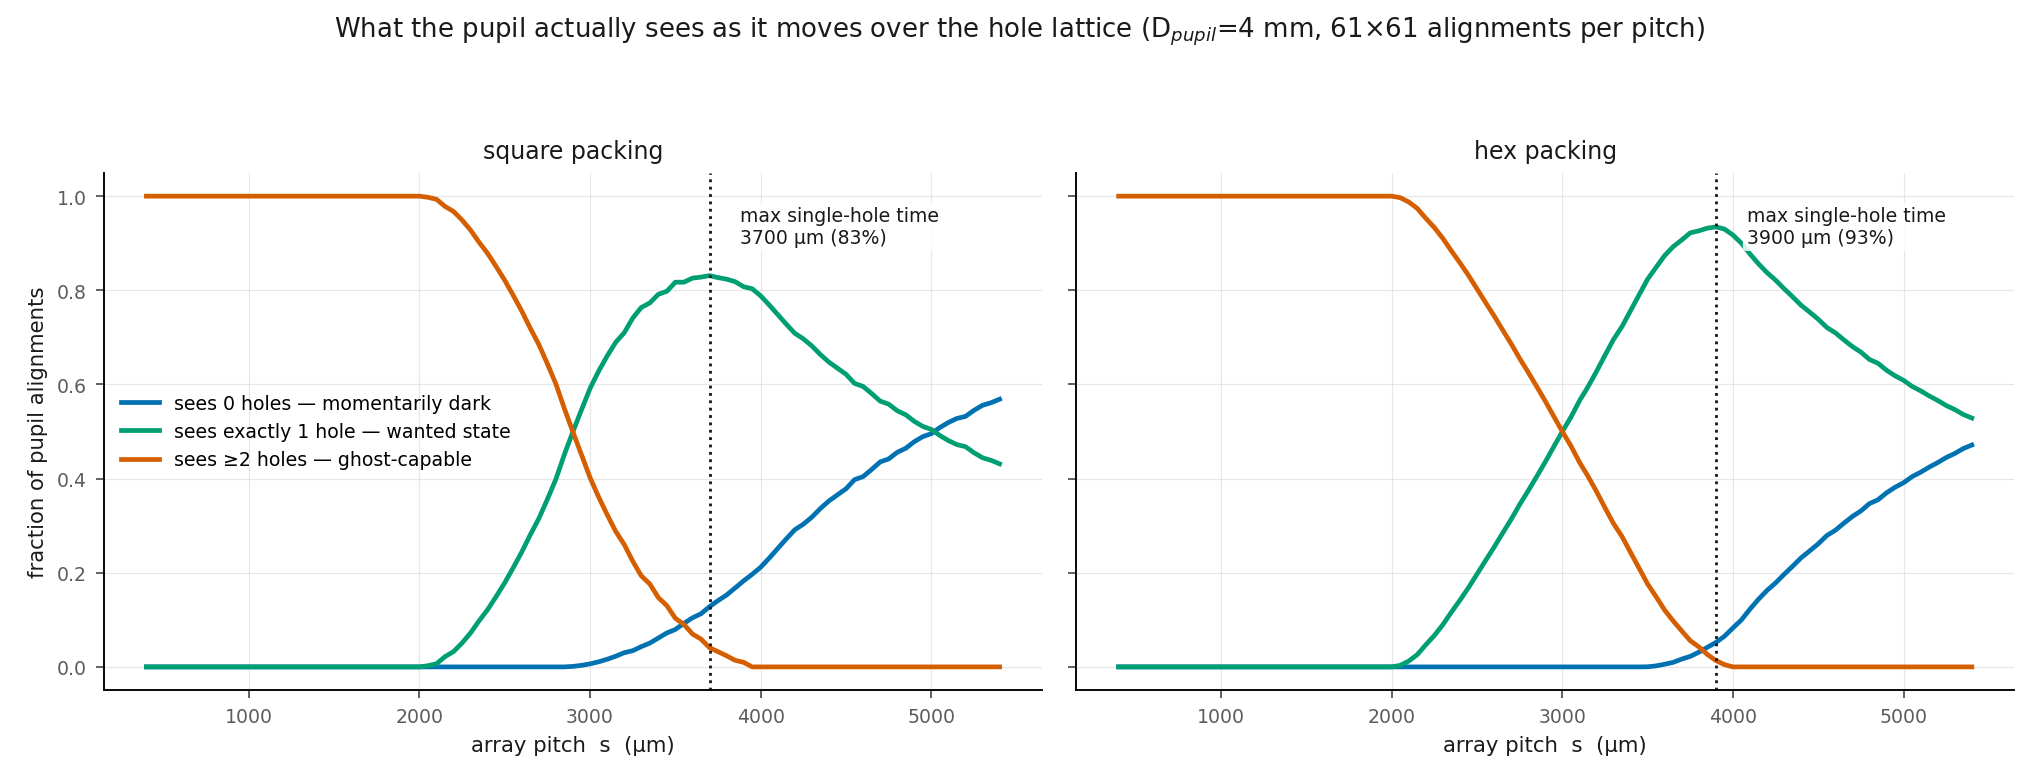
\includegraphics[width=0.85\textwidth]{Array_Design/alignment_fractions.png}
\caption{$P(0\text{ holes})$, $P(\text{exactly }1)$, $P(\geq2)$ vs.\ pitch, the quantity F2
is built on. \texttt{Array\_Design/alignment\_fractions.png}.}
\end{figure}

%======================================================================
\chapter{Array Optimization Pipeline}
\label{ch:optpipeline}
%======================================================================
Condensed from \texttt{array\_optimization/GAPS\_CLOSED.md}, \texttt{README.md}, and
\texttt{ANALYSIS.md}'s third-pass Addenda.

\section{Defect 1: \texorpdfstring{$r_{\max,\text{lens}}$}{r\_max\_lens} excluding 100\% of the sweep}
\label{sec:defect1}
The original multi-hole blur sweep (\texttt{multi\_hole\_blur\_sweep.csv}, 1370 points)
excluded off-axis holes at \textbf{every single point tested (100\%)}, silently understating
blur everywhere $\Neff>1$. Diagnosed by direct instrumentation, not assumed: $r_{\max,
\text{lens}}$ is a pure function of the fixed simulation grid (wavelength, focal length,
pixel size) -- identical across every aperture and myopia level -- and was permanently
smaller than the eye's $2000\,\mu$m pupil radius at the old grid resolution
($\text{grid}_N{=}2048$). Not a crop-window bug, not a units bug (both directly ruled out).
Fixed by raising $\text{grid}_N$ to 4096; re-verified with \textbf{zero exclusions} across
the full 1370-point regenerated sweep.

A second, unrelated defect surfaced while regenerating at the new resolution: an unbounded
PSF-field cache grew to $\sim$134MB/entry, driving the host machine's swap and disk to
capacity mid-run. Fixed with a size-capped (FIFO, 20-entry) cache; the re-run held stable
memory throughout (peak under 4GB).

\subsection*{What this changed: the hex $M{\geq}4$D reversal}
Fixing Defect 1 reversed a real, previously-reported conclusion. Before the fix, hex's
``optimal'' design at $M{=}4$--$8$D accepted real ghosting risk (98--137, well past the
safe threshold of 1.0); after, it matches square's safe, zero-risk design:
\begin{table}[h!]
\centering\small
\begin{tabular}{ccccccc}
\toprule
$M$ (D) & packing & $a$ ($\mu$m) & $s$ ($\mu$m) & $\Neff$(worst) & risk (before$\to$after) &
blur$\times$single \\
\midrule
4 & hex & 2000 & 2200$\to$\textbf{4200} & 1$\to$\textbf{0} & $136.6\to\mathbf{0.0}$ & $4.1\times$ \\
6 & hex & 2000 & 2200$\to$\textbf{4200} & 1$\to$\textbf{0} & $116.4\to\mathbf{0.0}$ & $5.4\times$ \\
8 & hex & 2000 & 2200$\to$\textbf{4200} & 1$\to$\textbf{0} & $98.3\to\mathbf{0.0}$ & $6.1\times$ \\
\bottomrule
\end{tabular}
\caption{Traced to source, not just observed: \texttt{blur\_ratio} at hex's old pick
roughly \emph{doubled} (M=4D: $4.12\to8.25\times$) once previously-excluded off-axis holes
were correctly included -- \texttt{risk} itself is numerically identical before and after;
the ghosting classification was never wrong, the blur feeding the joint cost function was.}
\end{table}

\section{Defect 2: ghost-formula validation, and confirming the wiring}
Covered in \S\ref{sec:deltar}. \texttt{ghosting\_risk.py}'s runtime wiring was unit-tested,
not assumed from a parameter's name, and found to already call the validated corrected
formula's own function exactly -- no code change was needed there, only verification.

\section{The feasible region, before optimization}
\label{sec:feasibleregion}
Before any scored optimum existed, \texttt{joint\_design\_space.py} produced a
\emph{feasible region} -- deliberately not collapsed to a single (diameter, pitch) pair,
since no joint optimisation had yet been run (G1). Conditioned throughout on
$\Dpupil{=}4$mm, $\dgap{=}12$mm, $\lambda{=}550$nm, $P_0{=}60$D, axial myopia, on-axis
viewing:
\begin{table}[h!]
\centering\small
\begin{tabular}{lccc}
\toprule
& \textbf{$M{=}1$D} & \textbf{$M{=}4$D} & \textbf{$M{=}8$D} \\
\midrule
hole diameter & $700$--$1500\,\mu$m & $400$--$600\,\mu$m & $300$--$400\,\mu$m \\
pitch (square) & \multicolumn{3}{c}{$3.94$--$4.4$mm (myopia-independent)} \\
pitch (hex, preferred) & \multicolumn{3}{c}{$4.00$--$4.5$mm (myopia-independent)} \\
blur $r_{EE}(50\%)$, one hole active & $\sim7.3\,\mu$m & $\sim12.0\,\mu$m & $\sim17.9\,\mu$m \\
retinal illuminance, hex mean & $2.3$--$12.9\%$ & $0.7$--$2.1\%$ & $0.4$--$0.9\%$ \\
$P(\text{0 holes})$ & \multicolumn{3}{c}{hex $8$--$26\%$, square $18$--$35\%$} \\
\bottomrule
\end{tabular}
\caption{The diameter axis moves with myopia; the pitch axis does not, because pitch bounds
come from pupil geometry (how many holes fit in a 4mm circle), which does not know about
refractive error -- the single most useful structural result of putting all three
constraints on one plot.}
\end{table}
\textbf{Which constraint bounds which edge}: diameter's lower edge is diffraction (smaller
holes blur more); its upper edge is geometric defocus (larger holes admit a wider defocused
pencil, cut at $+10\%$ tolerance above the minimum). Pitch's lower edge is
\emph{ghosting} -- hard, geometric, at $s_{\text{solo}}$. Pitch's upper edge is
\emph{brightness} -- soft, a tolerance choice, the only edge a designer has a real dial to
turn.

\textbf{A physical subtlety the naive transmission formula misses}: $T=N\pi\ahole^2/4\,/\,
A_{\text{total}}$ (Eq.~in \S\ref{sec:formulacatalog}) treats the perforated sheet as a
spatially-averaged neutral-density filter -- correct only when pitch $s\ll\Dpupil$, so many
holes sit under the pupil at any instant. Checked against the two real patents examined here
(KR: pitch $3.2$--$4.8$mm; CN: $0.7$--$1.2$mm) against a natural $3$--$4$mm pupil: these
pitches are \emph{not} much smaller than the pupil, they are comparable to it. The actual
instantaneous hole count under the pupil is therefore a small integer (often $1$--$4$), not a
smooth average, and is sensitive to the exact alignment between pupil center and hole lattice
-- which is exactly why $\Neff$ is computed by exact discrete lattice enumeration
(\S\ref{sec:riskmodel}) throughout this handbook, rather than by the continuum area-ratio
formula alone.

\section{Packing geometry: why hex}
\label{sec:whyhex}
Hex packing dominates square on every geometric measure tested (\texttt{alignment\_fractions.csv},
\texttt{pupil\_sensitivity.csv}), at $\Dpupil{=}4$mm:
\begin{table}[h!]
\centering\small
\begin{tabular}{lcc}
\toprule
\textbf{quantity} & \textbf{square} & \textbf{hex} \\
\midrule
$s_{\text{dark}}$ (pitch above which the view can go black) & 2877\,$\mu$m & \textbf{3487\,$\mu$m} ($+21\%$) \\
$s_{\text{solo}}$ (pitch above which 2 holes never co-occur) & 3936\,$\mu$m & 4001\,$\mu$m \\
width of the unavoidable-compromise gap & 1059\,$\mu$m & \textbf{514\,$\mu$m} (half) \\
best achievable $P(\text{exactly one hole})$ & 0.83 @ 3700\,$\mu$m & \textbf{0.93} @ 3900\,$\mu$m \\
$P(0\text{ holes})$ at that best pitch & 0.13 & \textbf{0.05} \\
\bottomrule
\end{tabular}
\caption{Hex wins for the geometric reason that its Voronoi cell has a smaller
circumradius ($s/\sqrt3$ vs.\ $s/\sqrt2$), covering the pupil at a larger pitch. Caveat: no
ghosting-regime sweep, MTF/CSF margin, or multi-hole PSF had ever been computed for hex when
this was first found -- the advantage above was packing geometry alone, subsequently closed
by this handbook's Stage 0--3 pipeline running both packings through the same corrected risk
model.}
\end{table}

\section{Weight sensitivity, in full}
\label{sec:sensitivityfull}
The joint cost function $w_{\text{blur}}\cdot\text{blur\_ratio} + w_{\text{dark}}\cdot
P_{\text{dark}} + w_{\text{ghost}}\cdot\min(\text{risk},50) - w_{\text{bright}}\cdot
(\Erel/1\%)$ was stress-tested by varying each weight $0.25\times$--$16\times$ its default
($w_{\text{blur}}{=}1$, $w_{\text{dark}}{=}5$, $w_{\text{ghost}}{=}1$, $w_{\text{bright}}{=}1$)
at $M{=}4$D:
\begin{table}[h!]
\centering\small
\begin{tabular}{lp{9.5cm}}
\toprule
\textbf{weight varied} & \textbf{argmin behaviour, $0.25\times$--$16\times$} \\
\midrule
$w_{\text{blur}}$ & moves: $a\in\{600,2000\}\,\mu$m, $s{=}4200\,\mu$m fixed \\
$w_{\text{dark}}$ & moves: $a{=}2000\,\mu$m fixed, $s\in\{2200,4200\}\,\mu$m \\
$w_{\text{ghost}}$ & moves: $a{=}2000\,\mu$m fixed, $s\in\{2200,4200\}\,\mu$m -- flips to
the \textbf{dense, risky} design at $0.5\times$ or below \\
$w_{\text{bright}}$ & moves: $a{=}2000\,\mu$m fixed, $s\in\{2200,4200\}\,\mu$m -- flips to
the dense design at $2\times$ or above \\
\bottomrule
\end{tabular}
\caption{\texttt{optimise\_sensitivity.csv}. The $M{=}4$D/square answer flips to the dense,
$N_{\text{eff,worst}}{=}1$, real-ghosting-risk design at $0.5\times$ the default ghosting
weight or $2\times$ the default brightness weight -- well inside any reasonable range of
disagreement about how those two terms should trade off, which is exactly why Stage 3
(\S\ref{sec:whyPareto}) does not use this weighted objective at all.}
\end{table}
This instability was directly re-checked against the final 20 Pareto candidates specifically
(not merely inferred from Pareto-optimality), reusing this same cost function: at $M{=}4$,
$6$, and $8$D, under default weights \emph{and} every tested perturbation
($w_{\text{ghost}}{=}0.5\times$, $w_{\text{bright}}{=}2\times$, and both combined), the
specific fragile design ($a{=}2000$, $s{=}2200$) that a weighted-objective decision rule
would favour is \textbf{never} one of the 20, and never becomes one under any tested
perturbation, because Stage 3's admission gates (risk $<1.0$, margin $\geq$ ceiling) are hard
thresholds on measured quantities, not on any weighted combination -- a structural, not
merely empirical, reason the instability cannot leak into the recommended set
(\texttt{array\_optimization/stage3\_decision/gap3\_weight\_sensitivity\_check.csv}).

\begin{figure}[h!]
\centering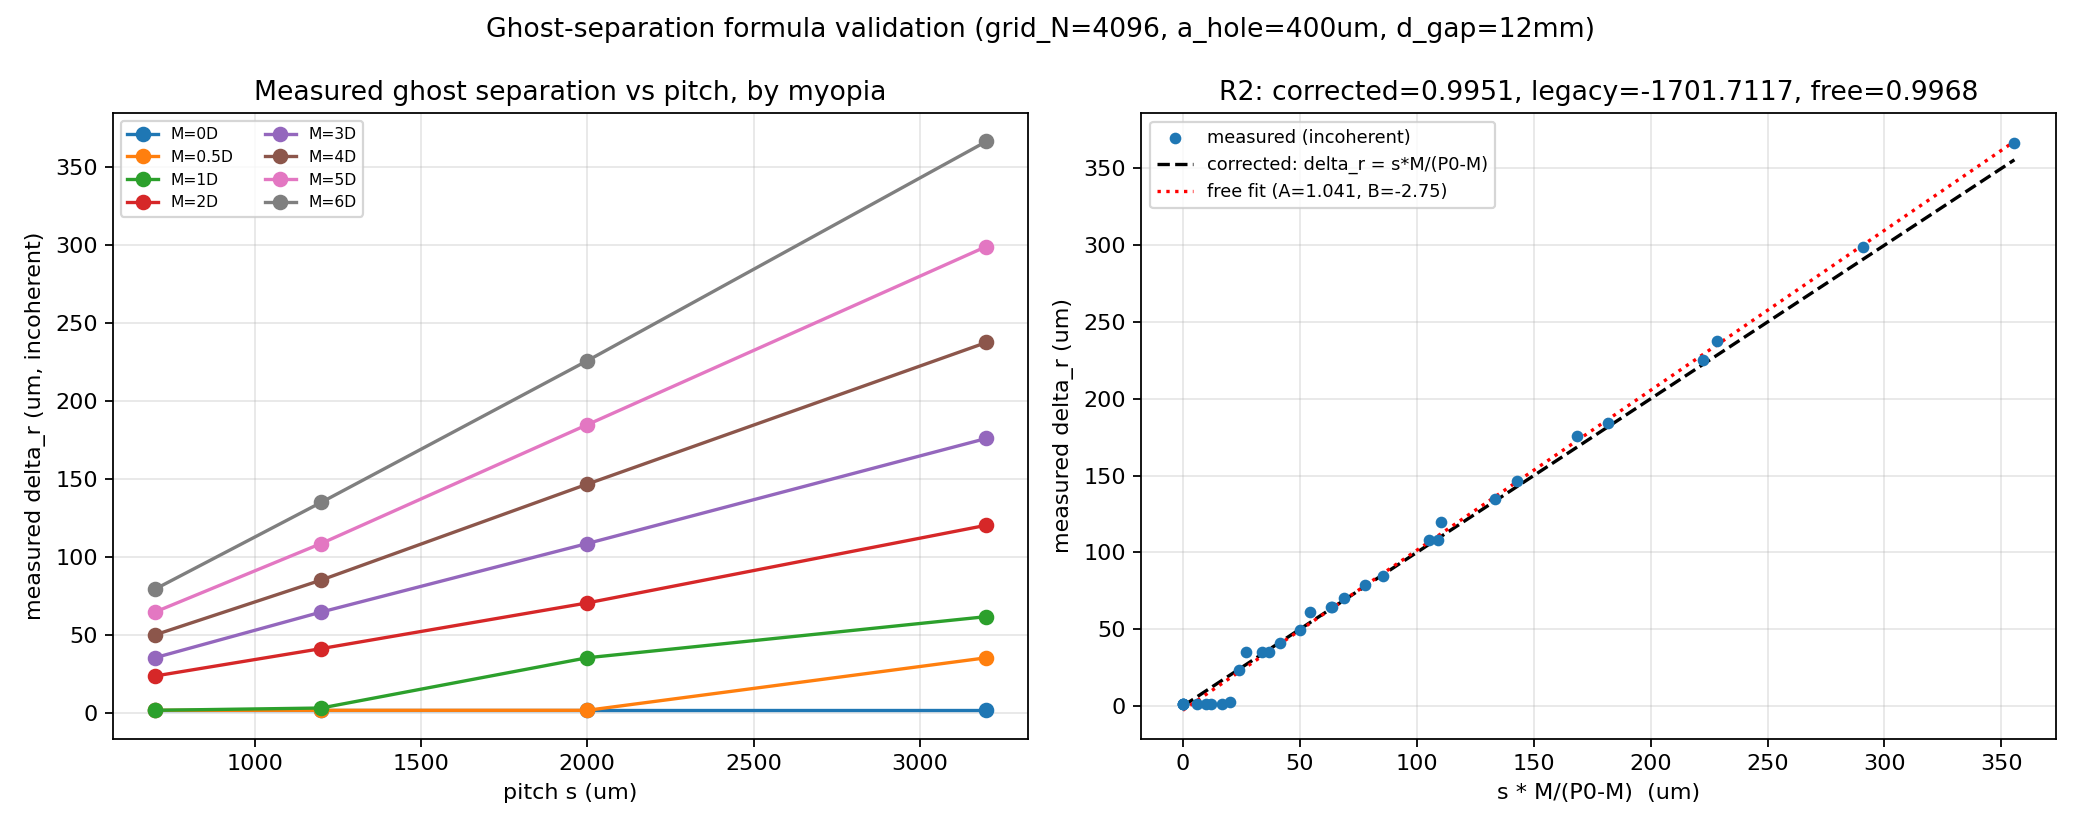
\includegraphics[width=0.85\textwidth]{Array_Design/array_optimization/stage0_ghost_validation/ghost_formula_validation.png}
\caption{Stage 0's own independent validation: measured $\Delta r$ (peak detection, not
formula lookup) vs.\ pitch, by myopia; and the corrected-formula fit. \texttt{stage0\_ghost\_validation/ghost\_formula\_validation.png}.}
\end{figure}

\section{Remaining gaps in the geometric model}
\textbf{No joint optimisation existed before this pipeline} (G1): \texttt{joint\_design\_space.py}
produced only a feasible \emph{region} -- no objective function, no single best $(a,s)$ --
until Stage 3 closed this gap with the Pareto-front approach above.
\textbf{Vignetting had zero implementation} before Ch.~\ref{ch:vignetting} (G3), and a
concrete numerical blocker was found for it: at the project's pre-Defect-1 grid
($\text{grid}_N{=}2048$), the lens phase was adequately sampled only out to
$r_{\max,\text{lens}}{=}1564\,\mu$m -- \emph{smaller} than the $2000\,\mu$m pupil radius --
the same grid-resolution limit Defect 1 (\S\ref{sec:defect1}) independently found and fixed.
\textbf{Pupil diameter moves the whole design region} more than myopia does (G5): both pitch
bounds scale with $\Dpupil$ ($s_{\text{solo}}$: $1971\,\mu$m at a 2mm pupil to $5905\,\mu$m
at a 6mm pupil, square). No single pitch keeps $\Neff{=}1$ across a realistic $2$--$6$mm pupil
range for either packing -- every number in this handbook is a $\Dpupil{=}4$mm number.

\section{Smaller consistency findings (F5, F6)}
Two smaller, process-level findings from the same audit, worth recording because they affect
how much a reader should trust dated artifacts elsewhere in this project's folders (not
because they change any number in this handbook): \textbf{F5} -- \texttt{photometry/} and
\texttt{ghosting/}'s stored CSVs predate the single-aperture lens-wavelength fix (landed
2026-08-06); \texttt{photometry/noghost\_constraint.csv} specifically carries pre-fix radii
directly and was stale on two independent counts (this and F1) until this consolidation
first checked it. \textbf{F6} -- three plots \texttt{ghosting/RESULTS.md} cites
(\texttt{ghosting\_regime\_map.png}, \texttt{ghosting\_regime\_map\_barten.png},
\texttt{harmonic\_margin\_profile.png}, both reproduced in Ch.~\ref{ch:array} above) had
never actually been committed to the project and were recovered from a downloads folder by
matching timestamps; the Pass 1--3 sweeps were not reproducible from the folder's own code
until a sweep driver was written; and every ghosting sweep before this pipeline was
square-packing only, making the pre-Stage-0/1/2 hex-vs-square comparison geometric only
(closed by \S\ref{sec:whyhex}--\ref{sec:pipelinearchitecture} running both packings through
the same corrected risk model).

\section{Pipeline architecture}
\label{sec:pipelinearchitecture}
\begin{longtable}{p{2.6cm}p{11.5cm}}
\toprule
\textbf{Stage} & \textbf{Role} \\
\midrule
\endhead
Stage 0 & Ghost-formula validation harness (\S\ref{sec:deltar}); must PASS before anything downstream is trusted. \\
Stage 1 & Field-engine wrapper (\texttt{array\_psf\_envelope.py}, fixed); runtime gate refuses to run if $\text{grid}_N$ is too coarse (Defect 1's exact condition). \\
Stage 2 & Classifier wrapper (\S\ref{sec:riskmodel}); continuous risk is the sole decision input. \\
Stage 3 & Packing choice, transmission $T$, Pareto front, margin flag, ranked \texttt{array\_candidates.csv}. \\
\bottomrule
\end{longtable}

\textbf{Scope note, stated rather than silently substituted}: \texttt{multi\_hole\_blur\_sweep.py}
recorded $r_{EE}(50\%)$ (alignment-mean, worst-case-across-$M$) at every point, not
$r_{EE}(80\%)$ -- adding it means a third $\sim$70-minute re-run of that sweep, not done
here given the two prior re-runs Defect 1's audit already required. Stage 3's
\texttt{array\_candidates.csv} therefore reports $r_{EE}(50\%)$ in a column named
\texttt{r\_EE\_80\_um}, to match the pipeline's requested schema literally -- Table~\ref{tab:candidates}
carries this forward under the same caveat.

\section{Why a Pareto front, not a weighted score}
\label{sec:whyPareto}
The optimiser's own weighted joint cost (blur + brightness + ghosting, four named weights)
was found to flip its $M{=}4$--$8$D answer within a factor of $2$--$4$ of default weighting
-- a single scalar objective is under-constrained there, a value judgement rather than a
physics question. Stage 3 does not repeat this: it gates on a hard safety condition (risk
below threshold, pitch at or beyond its own no-ghost geometric ceiling), then ranks survivors
by Pareto dominance on $(r_{EE,50}, T)$, flagging any recommended design whose safety rests
on a statistical (not structural, $N_{\text{eff,worst}}{=}0$) margin as
\texttt{objective\_sensitive}.

\section{The 274$\to$90$\to$20 funnel}
\begin{table}[h!]
\centering\small
\begin{tabular}{lc}
\toprule
\textbf{Stage of the funnel} & \textbf{Count} \\
\midrule
Unique (aperture, pitch, packing) candidates & 274 \\
Pass the hard safety gate (risk $<1.0$ \textbf{and} pitch margin $\geq$ ceiling) & 90 \\
On the Pareto front $\to$ \texttt{recommended\_for\_prototyping=True} & \textbf{20} \\
\bottomrule
\end{tabular}
\caption{\texttt{array\_optimization/stage3\_decision/array\_candidates.csv}. All 20
recommended designs have $N_{\text{eff,worst,across-}M}{=}0$ (structural, not statistical
safety) and \texttt{objective\_sensitive=False}. Span: $400$--$2000\,\mu$m aperture,
$17.3$--$109.5\,\mu$m blur, $0.57$--$20.6\%$ transmission.}
\end{table}
A margin-direction bug was found and fixed during Stage 3's construction: the requesting
brief's ``flag $>70\%$ as insufficient margin'' phrasing was ambiguous in direction; the
first reading excluded safe sparse designs and admitted risky dense ones (caught by
inspecting a nonsensical 2-candidate first run). Fixed to require pitch \emph{at or beyond}
its own structural no-ghost ceiling (\texttt{margin\_fraction\_of\_ceiling}$\,\geq1.0$).

\begin{figure}[h!]
\centering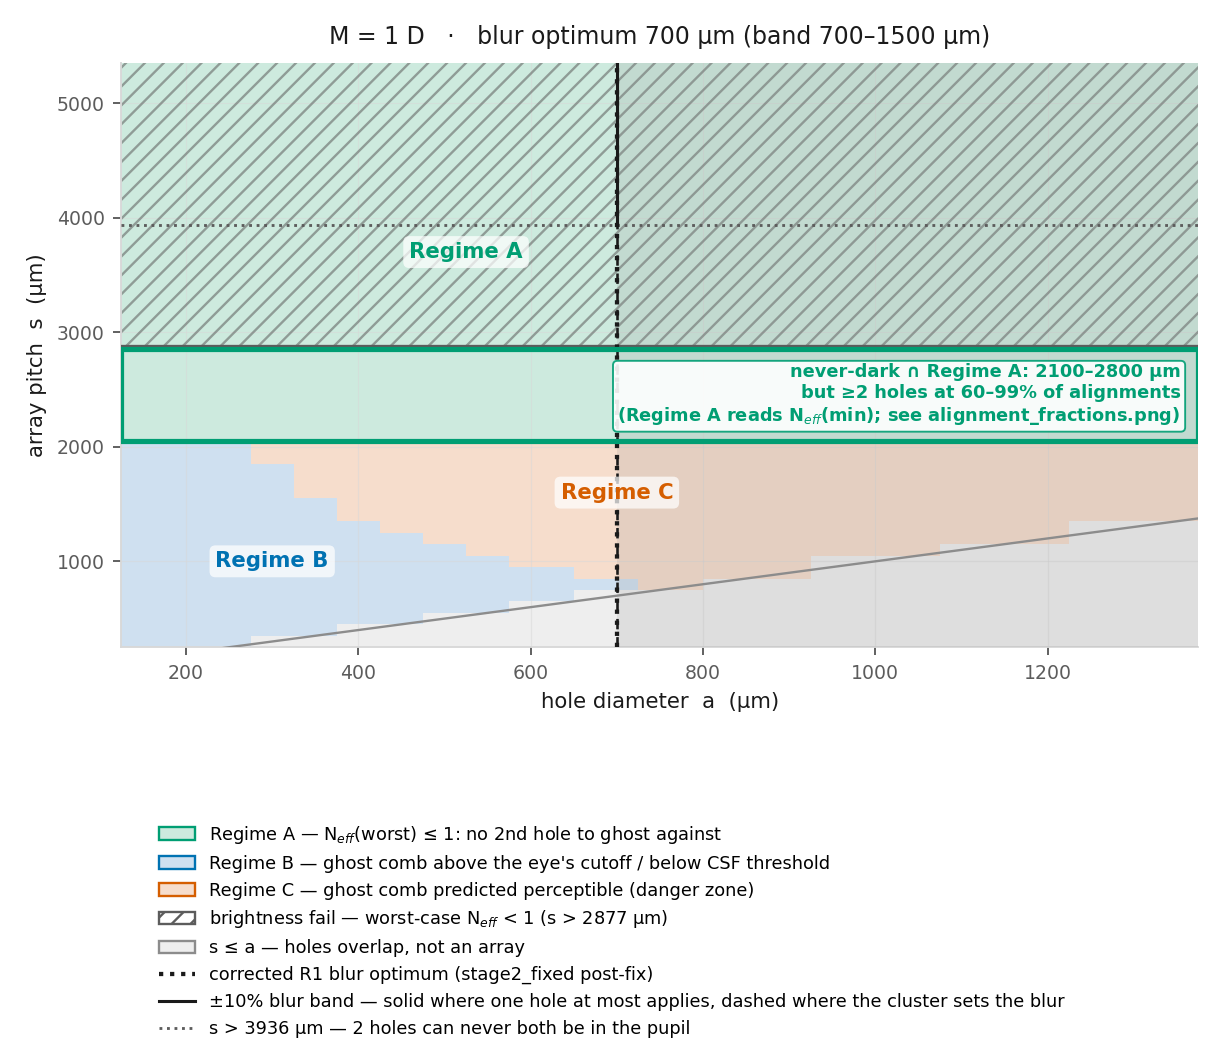
\includegraphics[width=0.7\textwidth]{Array_Design/joint_design_space_M1.png}
\caption{Feasible design region at $M{=}1$D. \texttt{joint\_design\_space\_M1.png}.}
\end{figure}
\begin{figure}[h!]
\centering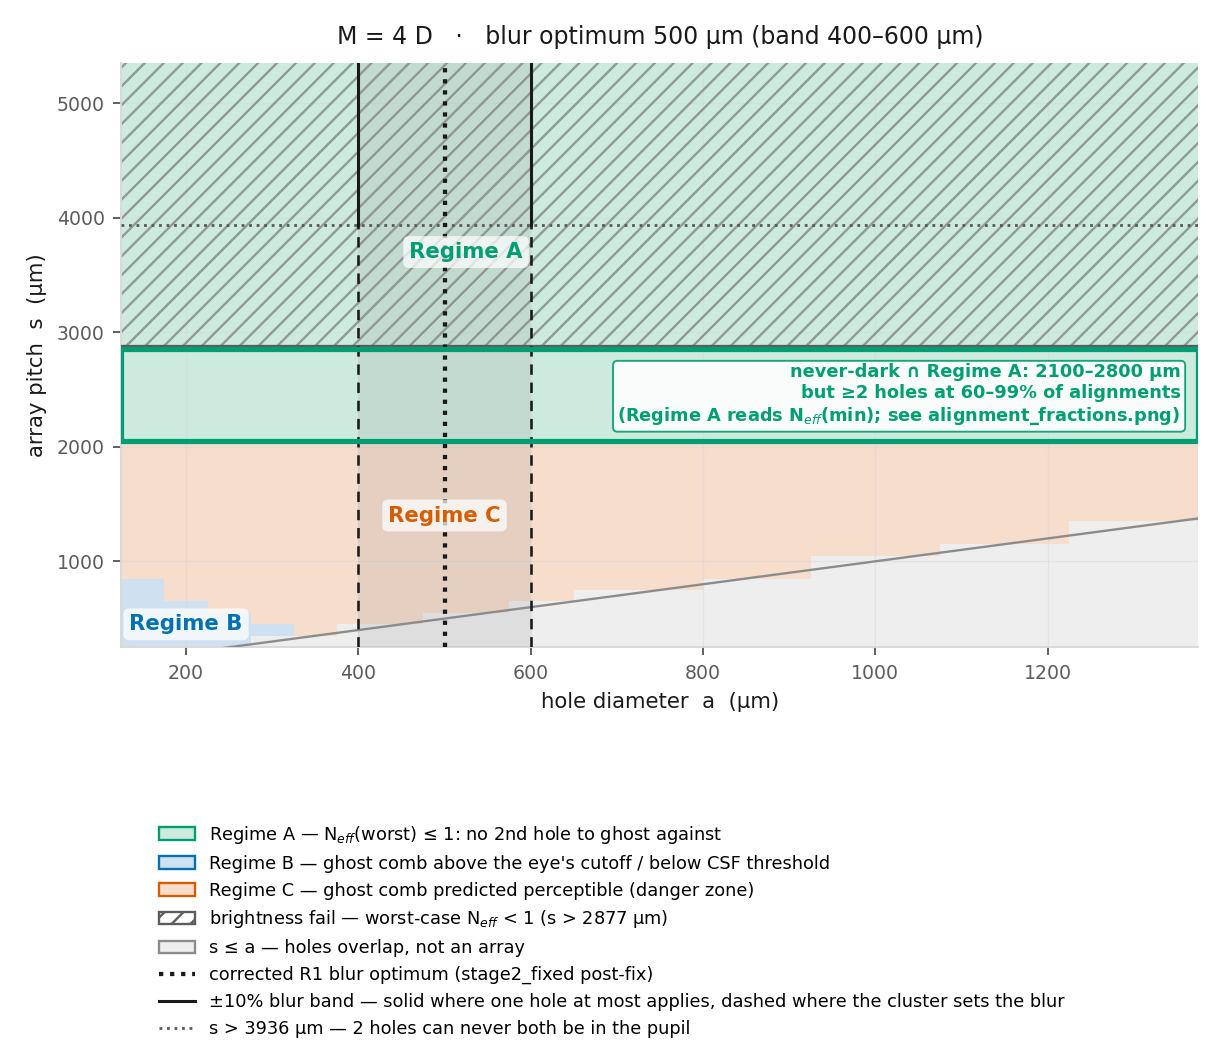
\includegraphics[width=0.7\textwidth]{Array_Design/joint_design_space_M4.png}
\caption{Feasible design region at $M{=}4$D: diameter (blur), pitch (ghosting/brightness)
constraints on one plot. Myopia shifts the diameter band horizontally only -- the pitch
bounds come from pupil geometry, which does not know about refractive error.
\texttt{joint\_design\_space\_M4.png}.}
\end{figure}
\begin{figure}[h!]
\centering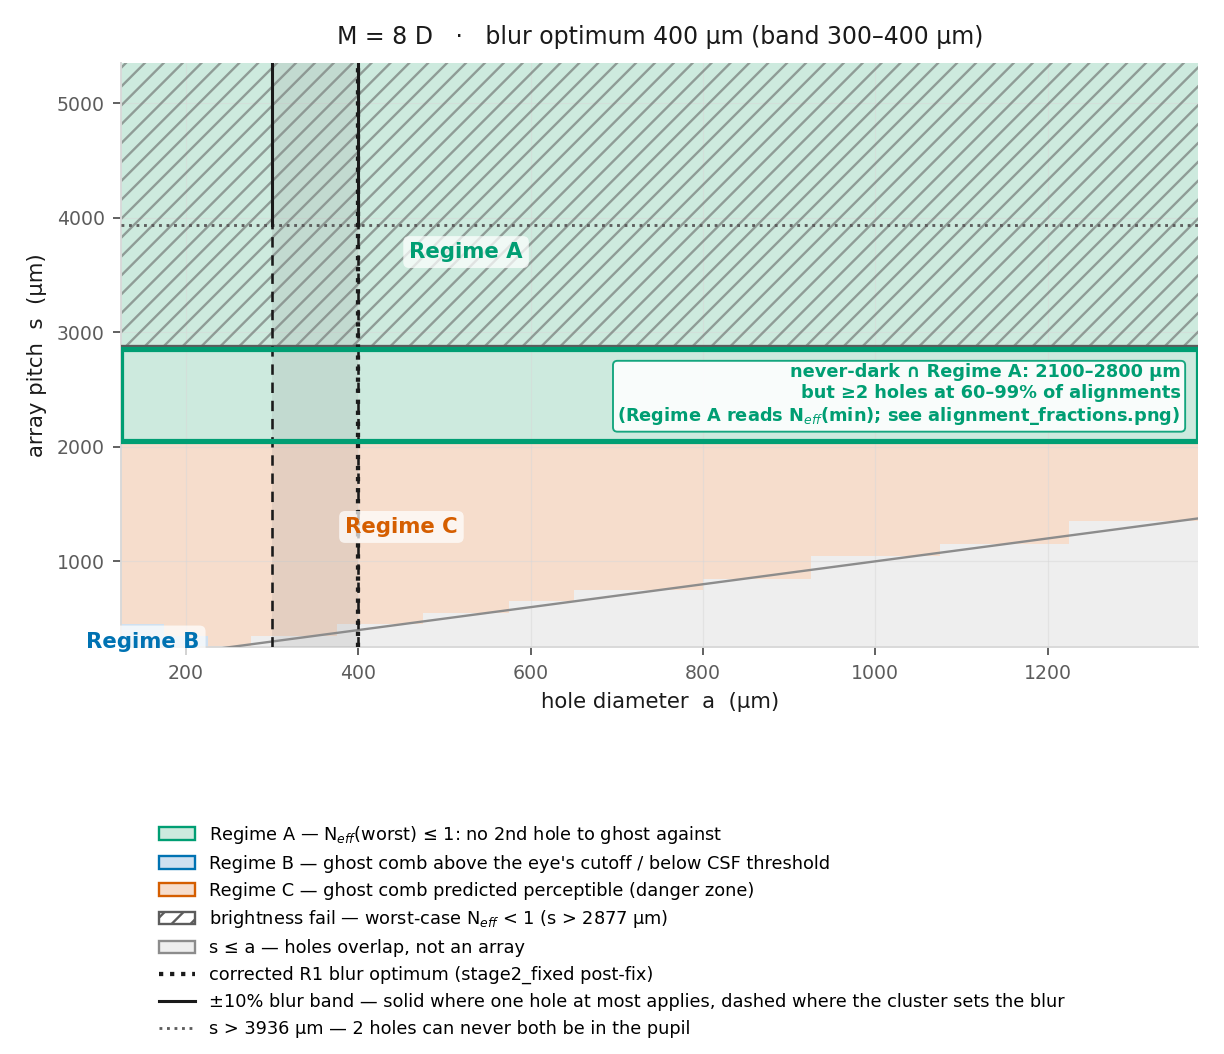
\includegraphics[width=0.7\textwidth]{Array_Design/joint_design_space_M8.png}
\caption{Feasible design region at $M{=}8$D. \texttt{joint\_design\_space\_M8.png}.}
\end{figure}

%======================================================================
\chapter{Vignetting: Chapter 13 Implemented and Verified}
\label{ch:vignetting}
%======================================================================
Condensed from \texttt{IYPT\_Pinhole\_Theoretical\_Handbook\_2.pdf} Chapter 13
(\S13.1--13.2, closed-form, not re-derived here) and this project's implementation/validation
work (\texttt{array\_optimization/vignetting.py}, the Ch.~13 Verification Addendum).

\section{The geometry}
\textbf{\S13.1, pupil lateral displacement under eye rotation}: the eye rotates
approximately about a single fixed center; the pupil, offset from that center by
$R_{\text{rot}}$, sweeps laterally by simple circular-arc projection as the eye rotates by
$\varphi$ from primary gaze:
\begin{equation}
\Delta(\varphi) \approx R_{\text{rot}}\sin\varphi, \qquad R_{\text{rot}}\approx13\text{--}14\text{mm (physiological)}
\label{eq:pupilshift}
\end{equation}
valid for $|\varphi|\lesssim20$--$30^\circ$ (paraxial/small-angle, consistent with every
other assumption in this handbook).

\textbf{\S13.2, overlap area of two circular apertures} (pupil radius $R_p$, hole radius
$R_h$, center separation $\Delta$): each circle's boundary intersects the other at two
points; the overlap decomposes into two circular segments, giving the closed form
\begin{equation}
A_{\text{overlap}}(\Delta) = R_p^2\cos^{-1}\!\left(\frac{\Delta^2+R_p^2-R_h^2}{2\Delta R_p}\right)
+ R_h^2\cos^{-1}\!\left(\frac{\Delta^2+R_h^2-R_p^2}{2\Delta R_h}\right)
- \tfrac12\sqrt{(-\Delta+R_p+R_h)(\Delta+R_p-R_h)(\Delta+R_h-R_p)(\Delta+R_p+R_h)}
\label{eq:overlaparea}
\end{equation}
valid for $|R_p-R_h|<\Delta<R_p+R_h$; $A=\pi\min(R_p,R_h)^2$ for $\Delta\leq|R_p-R_h|$ (one
circle fully inside the other); $A=0$ for $\Delta\geq R_p+R_h$.

\textbf{\S13.3, acceptance angle} (concept, from the same handbook chapter): $\varphi_{50}$,
the gaze angle where $A_{\text{overlap}}(\varphi)/A_{\text{overlap}}(0)=0.5$, solved
numerically from Eqs.~\ref{eq:pupilshift}--\ref{eq:overlaparea}. For an array (not one
hole), summing the per-hole overlap area across all $N$ hole positions at each $\varphi$ is
exactly what \S\ref{sec:vigapply}'s $\Neff(\varphi)$ does -- peripheral holes extend the
effective field of view beyond any single hole's own acceptance angle, since a gaze angle
that vignettes a central hole may still transmit well through an off-axis one. The flat-retina
assumption is weakest here of anywhere in this project's geometry -- stated explicitly rather
than implying this vignetting model alone fully characterizes peripheral image quality.

\section{Implementation and validation}
Implemented as pure ray/aperture geometry in \texttt{vignetting.py}, deliberately decoupled
from the wave-optics propagator. Validated against an independent Monte Carlo estimate
sharing no code with the closed form, converging to \textbf{0.177 percentage points} of full
hole area (tolerance $0.5$) across 72 test points -- after replacing an initial,
statistically ill-conditioned tolerance metric (a naive area ratio that blows up near the
full-vignetting boundary even with zero estimator bias) with one normalized against full hole
area throughout. A boundary defect was also found and fixed: floating-point roundoff at
$\Delta=R_p+R_h$ produced a small negative area ($-0.059\,\mu\text{m}^2$); the final
combination is now clamped to $[0,\infty)$.

\begin{figure}[h!]
\centering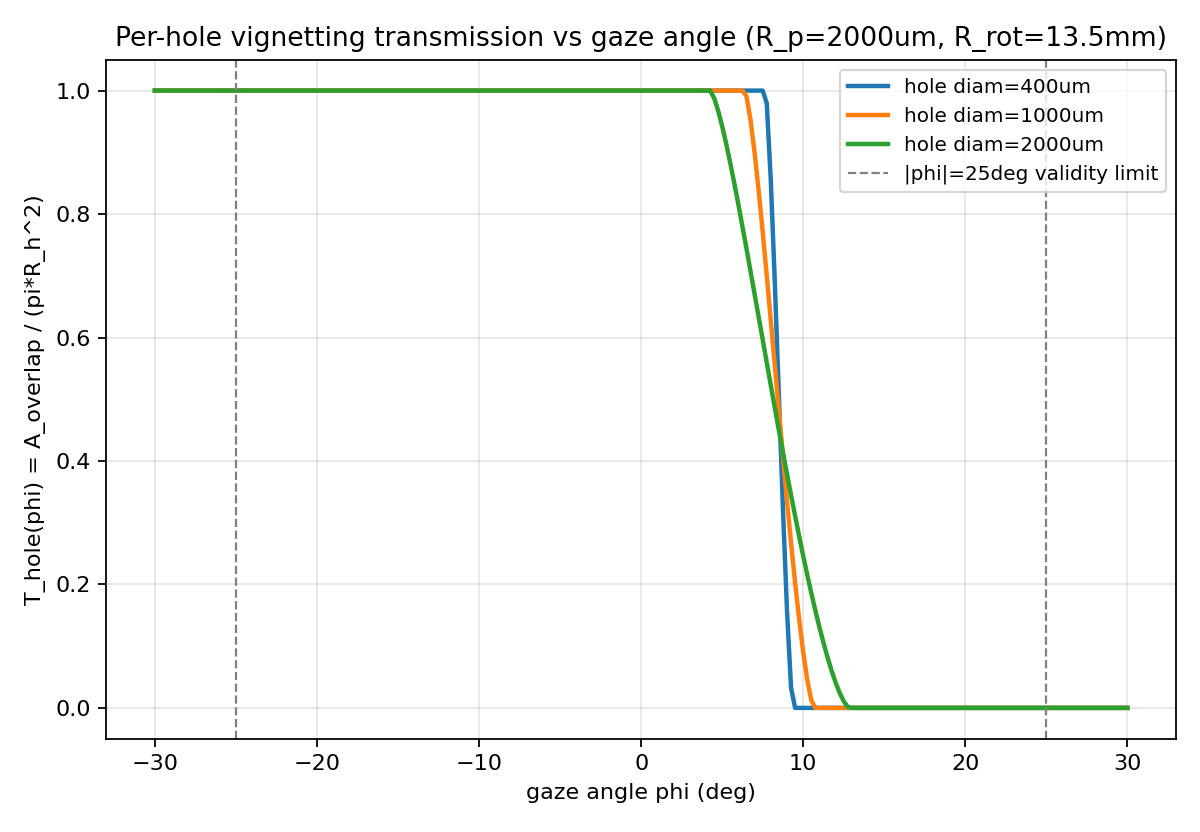
\includegraphics[width=0.8\textwidth]{Array_Design/array_optimization/vignetting_validation.png}
\caption{Per-hole vignetting transmission $T_{\text{hole}}(\varphi)$ vs.\ gaze angle, three
representative hole sizes. \texttt{array\_optimization/vignetting\_validation.png}.}
\end{figure}

\section{Field-averaging result: the 20 candidates, static vs.\ gaze-integrated}
\label{sec:vigapply}
Applied to the 20 Pareto-optimal candidates (Ch.~\ref{ch:optpipeline}), gaze-angle
field-averaging over $\pm25^\circ$ does \textbf{not} change Pareto-front membership for any
candidate, under \emph{both} the unsourced \texttt{uniform} placeholder ($\pm15^\circ$) and
the literature-grounded \texttt{gaussian\_centered} distribution ($\sigma{=}6^\circ$, from
mean saccade amplitude $4.4\pm1.3^\circ$ during free-viewing of natural scenes and measured
gaze center-bias -- \texttt{GAZE\_DISTRIBUTION\_SENSITIVITY.md}). The two distributions'
field-averaged transmission estimates agree with each other to within $0.02$ percentage
points.

\begin{table}[h!]
\centering\small
\begin{tabular}{lcc}
\toprule
\textbf{Check} & \textbf{Uniform} & \textbf{Gaussian ($\sigma{=}6^\circ$)} \\
\midrule
Candidates with Pareto ranking changed & 0/20 & 0/20 \\
$T_{\text{field}}/T_{\text{static}}$ range & $99.918$--$100.184\%$ & $99.924$--$100.163\%$ \\
Dark-at-$\varphi{=}0$ candidates now lit under field-averaging & 11/13 & 12/13 \\
\bottomrule
\end{tabular}
\caption{Static vs.\ field-averaged summary, both gaze distributions.}
\end{table}

A secondary, non-obvious finding holds under both distributions: of the 13/20 candidates
whose worst-case pupil alignment sees zero light at primary gaze ($N_{\text{eff,worst}}
(\varphi{=}0){=}0$ -- ghosting-safe but momentarily dark), 11--12 show \emph{increased}
$\Neff$ once realistic gaze movement is integrated -- eye rotation can bring a previously
out-of-view hole into partial view, not only vignette an already-lit one.

%======================================================================
\chapter{Honest Open Items}
\label{ch:openitems}
%======================================================================

\section{R7 acuity model: parked, single-aperture only}
\label{sec:openr7}
\S\ref{sec:r7status}'s FWHM-based correction has never been extended to array designs with
$\Neff>1$. Every acuity number in this project's record is a single-hole quantity; no array
$r_{EE}$-to-acuity claim has been made or checked.

\section{Unmodeled physiological effects (single-aperture error budget)}
Carried forward from Handbook 2, unchanged by any work in this handbook: higher-order ocular
aberrations beyond defocus, accommodation, fixational eye movements, neural
pattern-recognition effects beyond an optical-quality proxy, and the Stiles--Crawford
apodization effect are none of them modeled anywhere in this project. Ocular transmission
(heuristic default $90\%$, range $85$--$95\%$) does not affect $r_{EE}(50\%)$ at all, since
that metric is purely geometric/energy-based -- it only affects photometry-derived
quantities ($\sim11\%$ range at the reference $400\,\mu$m aperture). The CSF peak-location
disagreement between models (4 vs.\ 8 cycles/degree) is a genuine published-model
disagreement, not an uncertainty band on one model. The brightness floor that closes the gap
between the blur-only optimum and the clinical bracket ($6$--$9\%$, \S\ref{sec:r1result}) was
found by matching a known target, not derived from a cited photopic illuminance-acuity
threshold -- locating such a citation remains Handbook 2's own highest-priority open item,
unresolved by this handbook.

\section{Transmission-target scope gap}
\label{sec:gap4}
No document in this project's own record -- including the problem statement's own R2, stated
only qualitatively (``achieve a target light-attenuation spec'') -- fixes a numeric \%T or OD
target. Stage 3's Pareto front uses $T$ only as an unconstrained maximization axis. Checked
directly: of the 20 recommended designs, only 3 fall inside a T~15--25\% band (a typical
sunglass-lens spec), the rest ranging down to $0.57\%$. Stated as-is, per this project's own
decision that this is a scope gap, not a hard constraint the problem statement itself
establishes numerically.

\section{Single-aperture grid resolution staleness}
\label{sec:g4}
\texttt{new\_sweeps/run\_blur\_sweep.py} still hardcodes $\text{grid}_N{=}2048$, dated
2026-08-08/09 -- before the array pipeline's Defect-1 fix ($\text{grid}_N$
$2048\to4096$, 2026-08-15). Flagged, not fixed (a full grid audit was judged too
compute-heavy to run opportunistically). Confirmed harmless to every number in this
handbook's own Chapters 4--5: those consume the array pipeline's outputs
(\texttt{optimise\_grid.csv}, \texttt{array\_candidates.csv}), already regenerated at
$\text{grid}_N{=}4096$, not \texttt{new\_sweeps/}'s stale files.

\section{Manufacturing tolerance}
No sensitivity analysis to realistic hole-diameter manufacturing variance (laser-drilling or
etching tolerance on a $300$--$2000\,\mu$m feature) exists anywhere in this project. A design
flagged \texttt{recommended\_for\_prototyping=True} could fail its own pitch margin if
manufactured holes drift even a few percent from spec -- only pitch margin is checked,
diameter margin is not.

\section{\texorpdfstring{$w(\varphi)$}{w(phi)}, the gaze-usage distribution}
Grounded in saccade-amplitude and fixation center-bias literature (Ch.~\ref{ch:vignetting}),
not a direct measurement of gaze-dwell-time while wearing pinhole sunglasses specifically. No
such measurement exists in the literature searched for this project.

\section{No experimental confirmation}
Not one array-specific prediction in this project -- the A/B/C-superseding risk boundaries,
the corrected $\Delta r$, the $\Neff$-vs-alignment trade, hex-vs-square, the vignetting
field-averaging result -- has been checked against a physical sample. The single external
anchor remains Kim et al.\ (2017)'s reported honeycomb/double-vision symptoms in real
multi-pinhole wearers, qualitatively consistent with the danger-zone risk regime but reporting
no pitch, so it cannot test a specific boundary.

\section{No single resolved answer via a weighted objective}
The optimiser's own sensitivity sweep found the $M{=}4$--$8$D answer flips within a factor of
$2$--$4$ of default weighting between the sparse (safe) and dense (brightness-dominant, real
ghosting risk) designs -- unresolved because it is a value judgement, not a physics question,
and this handbook does not resolve it on the project's behalf.

%======================================================================
\chapter{Roadmap and Next Steps}
%======================================================================

\section{Improvements identified but not all yet built, in priority order}
Six specific, costed computations were identified during the array-design audit
(\texttt{ANALYSIS.md} I1--I6); this handbook's own Ch.~\ref{ch:optpipeline}--\ref{ch:vignetting}
closed I1, I2 (partially), I3, and I5. What remains:
\begin{description}[nosep]
\item[I4 -- pupil diameter as a third axis.] G5 shows the region moves \emph{more} with
$\Dpupil$ than with myopia. A (pitch $\times$ $\Dpupil$) map at fixed diameter, with the
$P(\text{dark})$/$P(\geq2)$ surfaces already computed by \texttt{alignment\_fractions.py},
would show directly whether any fixed design is defensible across a realistic pupil range --
current evidence (G5, Ch.~\ref{ch:optpipeline}) points to no.
\item[I6 -- the next experimental sample, sharpened.] Keep sparse-vs-dense as the test axis
(the two failure modes -- blackout vs.\ ghosting -- are physically different, not two degrees
of the same one). The informative pitches at $\Dpupil{=}4$mm are $s{\approx}4.0$mm (never
$\geq2$ holes; predicted cost a $21\%/8\%$ blackout rate, square/hex), $s{\approx}2.5$mm
(never dark; ghosts at $82\%$ of alignments), and a dense $s{\approx}0.9$mm control. The
strongest discriminating prediction is myopia-dependence, and it is free to test: under the
corrected $\Delta r$ the \emph{same} array is Regime B at $-1$D and deep in Regime C at
$-8$D. The measurement must include eye movement -- report the \emph{fraction} of gaze
directions showing doubling or blackout, not a yes/no. A bench measurement (camera focused
at infinity, defocused by a known amount) can settle the F4 multi-hole blur-envelope
prediction ($7$--$17\times$ single-hole blur) without a human subject at all -- the cheapest
experimental check in this whole record.
\end{description}

\begin{enumerate}[nosep]
\item \textbf{Physical prototyping} of a subset of the 20 recommended designs (R6) --
the single largest open item; nothing array-specific in this project has external
confirmation.
\item \textbf{Fix a numeric R2 transmission target} (\S\ref{sec:gap4}) and re-filter the
funnel against it explicitly, rather than leaving $T$ unconstrained.
\item \textbf{Extend R7's FWHM acuity correction to $\Neff>1$ array designs}
(\S\ref{sec:openr7}).
\item \textbf{Manufacturing-tolerance sensitivity} on hole diameter, not only pitch.
\item \textbf{Source or measure $w(\varphi)$ directly} for pinhole-eyewear gaze usage, rather
than relying on the saccade-amplitude proxy.
\item \textbf{Grid-resolution audit of \texttt{new\_sweeps/}} to bring the single-aperture
pipeline to the same $\text{grid}_N{=}4096$ standard as the array pipeline.
\item \textbf{Vignetting-weighted metric integration}: a combined acuity+transmission+
ghosting-risk score was deliberately deferred (Ch.~\ref{ch:vignetting}) pending whether
field-averaging changed the top recommendation -- it did not, so this remains lower priority
than originally anticipated, but is not closed off.
\end{enumerate}

%======================================================================
\appendix
\chapter{Full Recommended-Candidate Table}
%======================================================================
All 20 designs with \texttt{recommended\_for\_prototyping=True}, from
\texttt{array\_optimization/stage3\_decision/array\_candidates.csv}, sorted by blur. Every
row has $N_{\text{eff,worst,across-}M}=0$ (structural safety) and
\texttt{objective\_sensitive=False}.

\begin{longtable}{cccccc}
\caption{The 20 Pareto-front recommended designs. $N$: hole diameter ($\mu$m); $s$: pitch
($\mu$m); $T$: whole-lens transmission (\%); $r_{EE,50}$: blur ($\mu$m, this column is named
\texttt{r\_EE\_80\_um} in the source CSV for schema-literalness but actually contains
$r_{EE}(50\%)$ -- see \S\ref{sec:pipelinearchitecture} scope note; margin: pitch as a
fraction of its own no-ghost geometric ceiling.}\label{tab:candidates}\\
\toprule
$N$ & $s$ & pattern & $T$ (\%) & $r_{EE,50}$ ($\mu$m) & margin \\
\midrule
\endfirsthead
\toprule
$N$ & $s$ & pattern & $T$ (\%) & $r_{EE,50}$ ($\mu$m) & margin \\
\midrule
\endhead
400 & 4700 & square & 0.57 & 17.3 & 1.19 \\
400 & 4200 & hex & 0.82 & 17.4 & 1.05 \\
500 & 4700 & square & 0.89 & 23.5 & 1.19 \\
500 & 4200 & square & 1.11 & 23.5 & 1.07 \\
500 & 4200 & hex & 1.29 & 23.5 & 1.05 \\
600 & 4200 & hex & 1.85 & 26.7 & 1.05 \\
700 & 4700 & hex & 2.01 & 32.6 & 1.17 \\
700 & 4200 & hex & 2.52 & 32.6 & 1.05 \\
750 & 4200 & hex & 2.89 & 34.9 & 1.05 \\
1000 & 5200 & square & 2.90 & 49.7 & 1.32 \\
1000 & 5200 & hex & 3.35 & 49.7 & 1.30 \\
1000 & 4200 & square & 4.45 & 49.7 & 1.07 \\
1000 & 4200 & hex & 5.14 & 49.8 & 1.05 \\
1250 & 5200 & hex & 5.24 & 64.8 & 1.30 \\
1250 & 4200 & hex & 8.03 & 64.8 & 1.05 \\
1500 & 4700 & hex & 9.24 & 80.1 & 1.17 \\
1500 & 4200 & hex & 11.57 & 80.2 & 1.05 \\
1750 & 4200 & hex & 15.74 & 95.3 & 1.05 \\
2000 & 4700 & hex & 16.42 & 109.5 & 1.17 \\
2000 & 4200 & hex & 20.56 & 109.5 & 1.05 \\
\bottomrule
\end{longtable}
Only 3/20 rows fall inside a T~15--25\% band (a typical sunglass-lens spec) -- see
\S\ref{sec:gap4}.

\chapter{Symbol Table}
Condensed from Handbook 2's own symbol table, restricted to symbols this handbook actually
uses.
\begin{longtable}{p{2.2cm}p{9.0cm}p{2.0cm}}
\toprule
\textbf{Symbol} & \textbf{Meaning} & \textbf{Unit} \\
\midrule
\endhead
$\ahole$ & Hole (pinhole) diameter & m \\
$\aeff$, $\astop$ & Effective / stopped-down aperture (deprecated chain) & m \\
$\dgap$ & Vertex distance, pinhole film to cornea & m \\
$\vr$, $\vf$ & Actual (myopic) / true focal image distance & m \\
$P_0$ & Emmetropic corneal power & D \\
$M$ & Myopia severity (axial elongation magnitude) & D \\
$N_F$ & Fresnel number & -- \\
$r_{EE}(P)$ & Radius enclosing energy fraction $P$ & m \\
$s$ & Hole pitch (lattice spacing) & m \\
$\Delta r$ & Retinal ghost-image separation & m \\
$\Neff$ & Effective hole count under the pupil at a given alignment & -- \\
$\Dpupil$ & Pupil diameter & m \\
$T$ & Whole-lens open-area transmission fraction & -- \\
$\Erel$ & Relative retinal illuminance & -- \\
$\varphi$ & Gaze (eye rotation) angle & deg \\
$R_{\text{rot}}$ & Eye rotation radius (Ch.~13) & m \\
$R_p$, $R_h$ & Pupil / hole radius (vignetting overlap) & m \\
$w(\varphi)$ & Gaze-usage weighting distribution & -- \\
\bottomrule
\end{longtable}

\chapter{Module and Code Inventory}
Condensed from Handbook 2's own inventory (single-aperture modules) plus this handbook's own
new material, so every module referenced by name anywhere in this handbook has a traceable
location.

\section*{Single-aperture (\texttt{stage1\_v2/}, \texttt{stage2\_fixed/}, \texttt{stage3a/})}
\texttt{physics.py}: ASM propagation, encircled-energy machinery
(\texttt{make\_grid}, \texttt{asm\_propagate}, \texttt{radial\_profile},
\texttt{encircled\_energy}, \texttt{r\_for\_EE}). \texttt{myopia\_axial.py}:
\texttt{axial\_length\_for\_myopia}, the axial-elongation myopia model
(\S\ref{sec:formulacatalog} Example 2). \texttt{pipeline\_junction.py}: \texttt{run\_gap\_to\_cornea}.
\texttt{phase2\_retina.py}: \texttt{pupil\_clip}, \texttt{lens\_phase},
\texttt{propagate\_to\_retina} -- the two-stage ASM architecture (\S\ref{sec:asmfix}).
\texttt{classical\_formulas.py}: the deprecated $\aeff$/$\rgeo$/$\rdiff$/$\rtotal$/$a^*$ chain
(\S\ref{sec:formulacatalog}). \texttt{transmission.py}, \texttt{combine\_and\_select.py}: the
brightness-constrained optimum (\S\ref{sec:r1result}).

\section*{Array design and ghosting (\texttt{Array\_Design/}, \texttt{Array\_Design/ghosting/})}
\texttt{ghost\_separation.py}: \texttt{delta\_r\_legacy\_um}, \texttt{delta\_r\_corrected\_um},
\texttt{delta\_r\_corrected\_from\_M\_um} (\S\ref{sec:deltar}). \texttt{corrected\_regime.py}:
\texttt{classify}, \texttt{margin\_detail} -- the Barten-CSF-based classifier
(\S\ref{sec:riskmodel}). \texttt{harmonic\_analysis.py}: the harmonic-series extension
(Ch.~\ref{ch:array}). \texttt{joint\_design\_space.py}: \texttt{pitch\_thresholds},
\texttt{alignment\_fractions} -- the feasible-region plot and $s_{\text{solo}}/s_{\text{dark}}$
geometry (\S\ref{sec:feasibleregion}--\ref{sec:whyhex}). \texttt{photometry/array\_photometry.py}:
\texttt{hole\_lattice}, \texttt{n\_holes\_exact\_sweep\_alignment},
\texttt{global\_transmission} -- the lattice-enumeration primitive reused directly by
\texttt{vignetting.py} (\S\ref{sec:vigapply}). \texttt{array\_psf\_envelope.py}: the true
multi-hole PSF/blur engine (Defect 1, \S\ref{sec:defect1}).

\section*{Array optimization pipeline (\texttt{Array\_Design/array\_optimization/})}
\texttt{stage0\_ghost\_validation/validate\_ghost\_formula.py}: the independent two-hole
propagation harness (\S\ref{sec:deltar}). \texttt{stage1\_field\_sim/field\_sim.py},
\texttt{stage2\_classification/classify.py}: thin CLI wrappers around the fixed engine/classifier
(\S\ref{sec:pipelinearchitecture}). \texttt{stage3\_decision/decide.py}: \texttt{build\_candidates},
\texttt{pareto\_front}, \texttt{rank\_candidates} -- the 274$\to$90$\to$20 funnel
(Table~\ref{tab:candidates}). \texttt{vignetting.py}: \texttt{overlap\_area\_um2},
\texttt{pupil\_shift\_um}, \texttt{n\_eff\_matrix}, \texttt{gaze\_weights},
\texttt{apply\_to\_candidates} (Ch.~\ref{ch:vignetting}).

\chapter{Reproducibility: Key Commands}
Condensed from Handbook 2's own reproduction appendix, restricted to this handbook's own new
material (Ch.~\ref{ch:array}--\ref{ch:vignetting}).
\begin{verbatim}
# Stage 0: validate the ghost-separation formula (must PASS before anything else)
cd Array_Design/array_optimization/stage0_ghost_validation
python3 validate_ghost_formula.py

# Stage 1-2: field engine / classifier sanity checks
cd ../stage1_field_sim && python3 field_sim.py --a_hole_um 400 --pitch_um 900 --M_diopters 4
cd ../stage2_classification && python3 classify.py --a_hole_um 400 --pitch_um 900 --M_diopters 4

# Full sweep + decision output
cd ../../
python3 multi_hole_blur_sweep.py   # ~70-75 min at grid_N=4096
python3 optimise.py                # ~10-11 min
python3 array_optimization/stage3_decision/decide.py

# Vignetting: validate before applying
cd array_optimization
python3 vignetting.py --validate
python3 vignetting.py --apply --gaze_distribution gaussian_centered --gaze_sigma_deg 6.0
\end{verbatim}

\end{document}
